%%%%%%%%%%%%%%%%%%%%%%%%%%%%%%%%%%%%%%%%%%  不使用 authblk 包制作标题  %%%%%%%%%%%%%%%%%%%%%%%%%%%%%%%%%%%%%%%%%%%%%%
%-------------------------------PPT Title-------------------------------------
\title{计算材料模拟软件与优化}
%-----------------------------------------------------------------------------

%----------------------------Author & Date------------------------------------
%\author[\textrm{Jun\_Jiang}]{姜\;\;骏\inst{}} %[]{} (optional, use only with lots of authors)
%% - Give the names in the same order as the appear in the paper.
%% - Use the \inst{?} command only if the authors have different
%%   affiliation.
\institute[BCC]{\inst{}%
%\institute[Gain~Strong]{\inst{}%
\vskip -20pt 北京市计算中心~云平台事业部~姜骏}
%\vskip -20pt {\large 格致斯创~科技}}
\date[\today] % (optional, should be abbreviation of conference name)
{	{\fontsize{6.2pt}{4.2pt}\selectfont{\textcolor{blue}{E-mail:~}\url{jiangjun@bcc.ac.cn}}}
\vskip 45 pt {\fontsize{8.2pt}{6.2pt}\selectfont{%北京科技大学% 报告地点
	\vskip 5 pt \textrm{2024.06.20}}}
}

%% - Either use conference name or its abbreviation
%% - Not really information to the audience, more for people (including
%%   yourself) who are reading the slides onlin%%   yourself) who are reading the slides onlin%%   yourself) who are reading the slides onlineee
%%%%%%%%%%%%%%%%%%%%%%%%%%%%%%%%%%%%%%%%%%%%%%%%%%%%%%%%%%%%%%%%%%%%%%%%%%%%%%%%%%%%%%%%%%%%%%%%%%%%%%%%%%%%%%%%%%%%%

\subject{}
% This is only inserted into the PDF information catalog. Can be left
% out.
%\maketitle
\frame
{
%	\frametitle{\fontsize{9.5pt}{5.2pt}\selectfont{\textcolor{orange}{“高通量并发式材料计算算法与软件”年度检查}}}
\titlepage
}
%-----------------------------------------------------------------------------

%------------------------------------------------------------------------------列出全文 outline ---------------------------------------------------------------------------------
%\section*{}
%\frame[allowframebreaks]
%{
%  \frametitle{Outline}
%%  \frametitle{\textcolor{mycolor}{\secname}}
%  \tableofcontents%[current,currentsection,currentsubsection]
%}
%%在每个section之前列出全部Outline
%%类似的在每个subsection之前列出全部Outline是\AtBeginSubsection[]
%\AtBeginSection[]
%{
%  \frame<handout:0>%[allowframebreaks]
%  {
%    \frametitle{Outline}
%%全部Outline中,本部分加亮
%    \tableofcontents[current,currentsection]
%  }
%}

%-----------------------------------------------PPT main Body------------------------------------------------------------------------------------
\small
%\section{引言}
\frame
{
	\frametitle{\rm{I~Have~A~Dream}}
\begin{figure}[h!]
\vspace*{-0.18in}
\centering
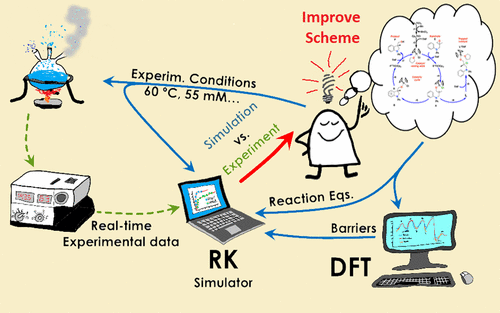
\includegraphics[height=2.55in,width=4.05in]{Figures/Schematic_Material-Design.png}
%\caption{\tiny \textrm{Pseudopotential for metallic sodium, based on the empty core model and screened by the Thomas-Fermi dielectric function.}}%(与文献\cite{EPJB33-47_2003}图1对比)
%\caption{\tiny \textrm{Pseudopotential for metallic sodium, based on the empty core model and screened by the Thomas-Fermi dielectric function.}}%(与文献\cite{EPJB33-47_2003}图1对比)
\label{Schematic_Material-Design}
\end{figure} 
}

\frame
{
%\documentclass[tikz,svgnames,border={0 2}]{standalone}
%\renewcommand\vec[1]{\boldsymbol{#1}}
%\begin{document}
\begin{tikzpicture}[
    box/.style={rectangle,draw,fill=DarkGray!20,node distance=1cm,text width=15em,text centered,rounded corners,minimum height=2em,thick},
    box1/.style={rectangle,draw,fill=green!50,node distance=1cm,text width=12em,text centered,rounded corners,minimum height=2em,thick},
    box2/.style={rectangle,draw,fill=magenta!75,node distance=1cm,text width=12em,text centered,rounded corners,minimum height=2em,thick},
    box3/.style={rectangle,draw,fill=blue!30,node distance=1cm,text width=12em,text centered,rounded corners,minimum height=2em,thick},
    box4/.style={rectangle,draw,fill=violet!45,node distance=2cm,text width=13em,text centered,rounded corners,minimum height=2em,thick},
%    arrow/.style={draw,-latex', thick},
    arrow/.style={draw,-latex', red, line width=2pt},
  ]
%  \node [box] (potential) {$v_{\text{ext},s}(\vec r)=v_\text{H}(\vec r) + v_\text{xc}(\vec r) + v_\text{ext}(\vec r)$};
  \node [box1,text width=8em] (Softwares) {实际程序\\实现和应用};
%  \node [box,below=0.5 of potential] (hamiltonian) {$\hat{H}_{KS}=-\frac{\hbar^2}{2m}\vec{\nabla}^2 + v_{\text{ext},s}(\vec r)$};
  \node [box2,below=0.5 of Softwares] (Method) {基组和势函数处理方法\\$\vec k$空间积分方案};
%  \node [box,below=0.5 of hamiltonian] (se) {$\hat{H}_{KS} \phi_i(\vec r)= E_i \phi_i(\vec r)$};
  \node [box3,below=0.7 of Method, text width=13em] (Theory) {基本理论\\\textrm{DFT}和\textrm{Band Structure}};
%  \node [box,below=0.5 of se] (density) {$\rho(\vec r)=\sum_{i=1}^n f_i\,|\phi_i(\vec r_i)|^2$};
  \node [box4,below=0.8 of Theory, text width=15em] (Basic-Equ) {(学科)基本方程\\量子力学:~\textrm{Schr\"odinger}方程\\$\hat{\mathbf H}\Psi=E\Psi$};
%  \node [box,below=0.5 of density] (criterion) {Convergence criterion satisfied?};

%  \node [box,above=1.5 of potential, fill=orange!30, text width=20em] (initial) {Supply initial density guess $\rho_\text{ini}(\vec r)$ to Kohn Sham equations};
  \node [box4,left=0.5 of Basic-Equ, fill=violet!30, text width=5em, minimum height=5em] (PDE) {经典数值\\分析算法};
%  \node [box,below=1.5 of criterion, fill=blue!30, text width=20em] (energy) {Use $\rho_\text{fin}(\vec r)$ to minimize total energy functional $E_{V_\text{ext}}[\rho]=T_{e,s}[\phi_i\{\rho\}] + V_{ee,H}[\rho] + E_{xc}[\rho] + V_{eI}[\rho]$};
  \node [box4,left=1.0 of Method, fill=magenta!50, text width=5em] (Algorithm) {具体\\算法\\实现};

  \node [box4,right=0.5 of Basic-Equ, fill=violet!30, text width=5em] (OS) {操作\\系统\\与\\编程\\技术};
  \node [box4,right=1.0 of Method, fill=magenta!50, text width=5em] (coding) {程序语言};
%  \node [box4,right=1.0 of Method, fill=magenta!50, text width=5em, draw=red, thick] at (-5,0) (Figure) {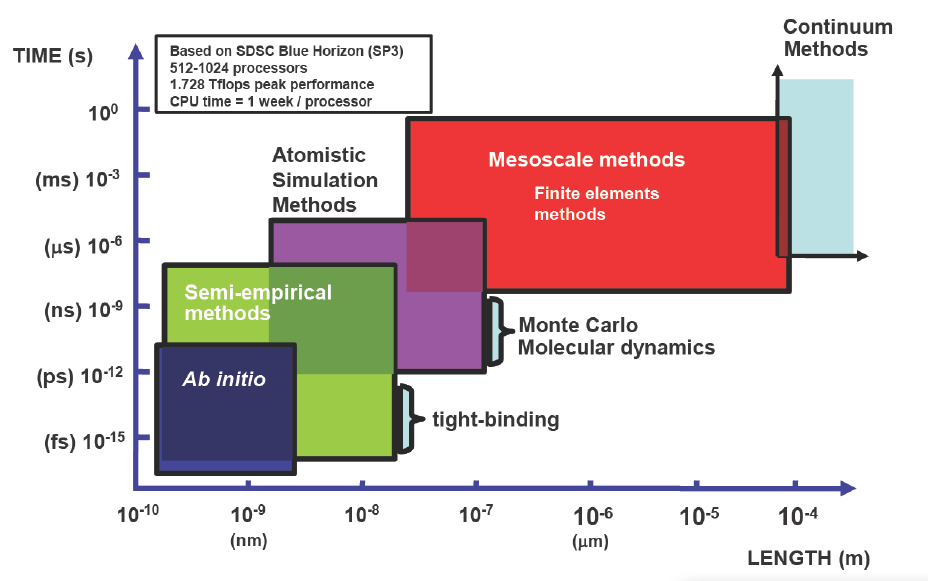
\includegraphics[width=0.5in, height=0.4in]{Figures/Multi-Scale-6.png}};
%  \path [arrow] (initial) -- (potential);
  \path [arrow] (Method) -- (Softwares);
  \path [arrow] (Theory) -- (Method);
  \path [arrow] (Basic-Equ) -- (Theory);
%  \path [arrow] (density) -- (criterion);

  \path [arrow] (PDE) -- (Algorithm);
  \path [arrow] (OS) -- (coding);
 % \path [arrow] (OS) -- (Figure);
  \path [arrow] (coding) |- (Softwares.east);
  \path [arrow] (Algorithm) |- (Softwares.west);
  \path [arrow] (Method.east) -- (coding.west);
  \path [arrow] (Method.west) -- (Algorithm.east);

%%%%%% ------------ 定义 虚线方框转角 -----------------  %%%%%%
%  \path
%  (potential.north west) ++(-1em,1em) coordinate (potential fit)
%  (criterion.south east) ++(1em,-1em) coordinate (criterion fit);

%%%%%% ------------ 绘制 虚线方框 -----------------  %%%%%%
%  \node [rectangle,draw,dashed,inner sep=1em,fit=(potential fit) (criterion fit)] (enclosure) {};
%  \node [above=-0.8em of enclosure,anchor=south,draw,outer sep=0pt,fill=white] (enclosure label) {\Large\textbf{Kohn-Sham method}};

%  \path [arrow] (criterion) -- (energy) node [midway,left=0.1,draw,outer sep=0pt,fill=white] (TextNode) {Yes};
%  \path [draw,thick] (criterion.south) ++(0em,-1em) -- (criterion fit) node [midway,below=0.1,sloped,draw,outer sep=0pt,fill=white] (TextNode) {No};
%  \draw [arrow] (criterion fit) |- (potential.east);
\end{tikzpicture}
}

\frame
{
%	\frametitle{\textrm{DFT-SCF}}
\begin{figure}[h!]
\vspace*{-0.25in}
\centering
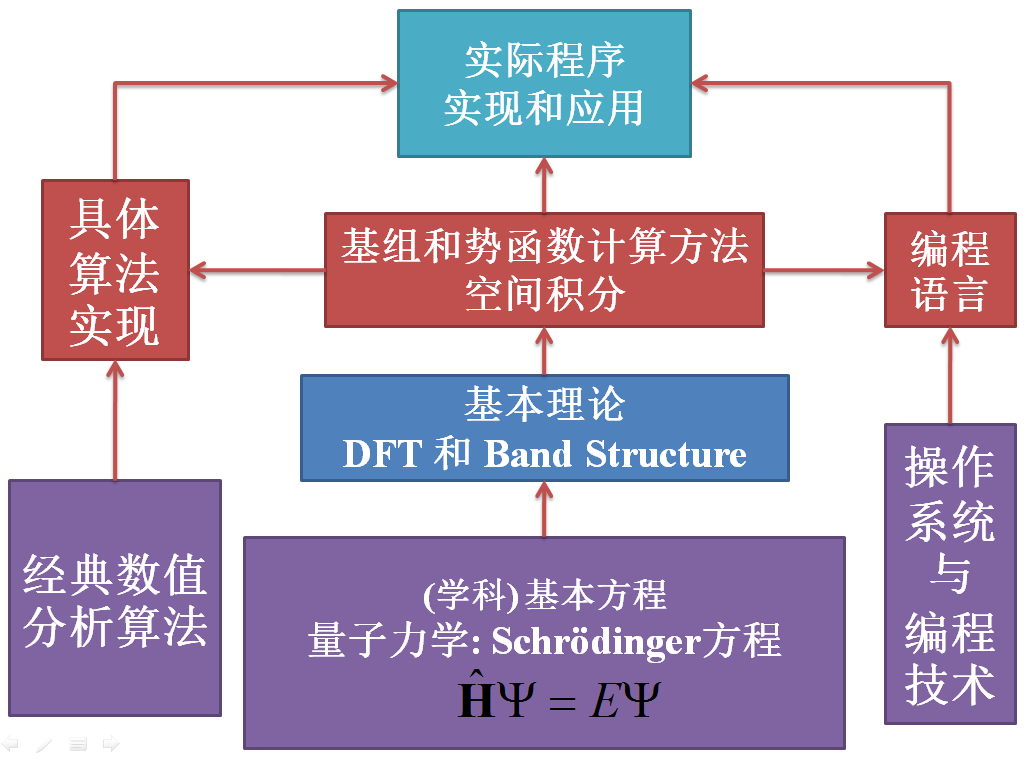
\includegraphics[height=2.80in,width=4.95in,viewport=5 3 1250 780,clip]{Figures/Method_Procedure.png}
%\caption{\tiny \textrm{Pseudopotential for metallic sodium, based on the empty core model and screened by the Thomas-Fermi dielectric function.}}%(与文献\cite{EPJB33-47_2003}图1对比)
\label{Method-Procedure}
\end{figure}
}

%-----------------------------------------------------------------------------------------------------------------------------------------------------------------------%
\frame
{
%\documentclass[tikz,svgnames,border={0 2}]{standalone}
%\renewcommand\vec[1]{\boldsymbol{#1}}
%\begin{document}
\begin{tikzpicture}[
    box/.style={rectangle,draw,fill=darkgray!20,node distance=1cm,text width=15em,text centered,rounded corners,minimum height=2em,thick},
    box1/.style={diamond, aspect=7, inner sep=2pt, draw,fill=green!50,node distance=1cm,text width=12em,text centered,rounded corners,minimum height=2em,thick},
    box2/.style={rectangle,draw,fill=magenta!75,node distance=1cm,text width=12em,text centered,rounded corners,minimum height=2em,thick},
    box3/.style={rectangle,draw,fill=blue!30,node distance=1cm,text width=12em,text centered,rounded corners,minimum height=2em,thick},
    box4/.style={rectangle,draw,fill=violet!45,node distance=2cm,text width=13em,text centered,rounded corners,minimum height=2em,thick},
%    arrow/.style={draw,-latex', thick},
    arrow/.style={draw,-latex', red, line width=2pt},
  ]
%  \node [box] (potential) {$v_{\text{ext},s}(\vec r)=v_\text{H}(\vec r) + v_\text{xc}(\vec r) + v_\text{ext}(\vec r)$};
  \node [box, fill=brown!80, text width=2.5em, minimum height=1em] at(-10,2) (Symmetry-OP) {\fontsize{6.0pt}{4.5pt}\selectfont{对称操作}};
  \node [box, fill=blue!30, text width=7.0em, minimum height=1em] at(-7.5,2.4) (Init-Wave) {\fontsize{6.0pt}{4.5pt}\selectfont{初始结构~(经验或猜测)}};
  \node [box, fill=blue!30, text width=5.0em, minimum height=1em] at(-7.5,1.6) (Init-charge) {\fontsize{6.0pt}{4.5pt}\selectfont{初始电荷密度$\rho_0$}};
  \node [box, draw=blue, fill=white, text width=8.0em, minimum height=1em] at(-4.0,1.8) (DFT-SCF) {\fontsize{16.0pt}{4.5pt}\selectfont{\textcolor{blue}{\bf{DFT-$SCF$}}}};
  \node [box, below=0.6 of Symmetry-OP, fill=blue!120, text width=5.0em, minimum height=1em] (Potential) {\fontsize{6.0pt}{4.5pt}\selectfont{\textcolor{white}{全势\textrm{(FP)}方法\\赝势\textrm{(PP)}方法}}};
  \node [box, right=0.2 of Potential, fill=blue!60, text width=6.0em, minimum height=1em] (Hartree) {\fontsize{6.0pt}{4.5pt}\selectfont{\textrm{Hartree}势$V_\mathrm{H}(\vec r)$}};
  \node [box, right=0.8 of Hartree, fill=blue!60, text width=7.0em, minimum height=1em] (Exch-Cor) {\fontsize{6.0pt}{4.5pt}\selectfont{交换-相关势$V_{\mathrm{XC}}[\rho(\vec r)]$}};
  \node [box, below=0.2 of Potential, fill=orange!80, text width=7.0em, minimum height=1em] (Basis-set) {\fontsize{6.0pt}{4.5pt}\selectfont{基函数}};
  \node [box, right=1.1 of Basis-set, fill=red!80, text width=7.0em, minimum height=1em] (Fock-matrix) {\fontsize{6.0pt}{4.5pt}\selectfont{构造\textrm{Fock}矩阵}};
  \node [box, below=0.2 of Fock-matrix, fill=green!80, text width=7.0em, minimum height=1em] (Kohn-Sham) {\fontsize{6.0pt}{4.5pt}\selectfont{求解\textrm{Kohn-Sham}方程(\textrm{Fock}矩阵对角化)}};
  \node [box, below=0.2 of Kohn-Sham, fill=blue!80, text width=7.0em, minimum height=1em] (Wave-Eigen) {\fontsize{6.0pt}{4.5pt}\selectfont{本征态波函数$\Psi_i(\vec r)$,能量本征值$\varepsilon_i$}};
  \node [box, draw=blue, fill=white, text width=5.0em, minimum height=1em] at(-2.0,-2.7) (k-space) {\fontsize{6.0pt}{4.5pt}\selectfont{$\vec k$-空间积分方案}};
  \node [box, below=0.2 of Wave-Eigen, fill=blue!80, text width=7.0em, minimum height=1em] (Charge) {\fontsize{6.0pt}{4.5pt}\selectfont{计算电荷密度$\rho$}};
  \node [box, below=3.0 of Basis-set, fill=blue!80, text width=4.6em, minimum height=1em] (Ion-Static) {\fontsize{4.0pt}{4.5pt}\selectfont{离子静电作用$E_{\mathrm{N-N}}$}};
  \node [box, right=0.05 of Ion-Static, fill=blue!80, text width=5.5em, minimum height=1em] (Ion-ele) {\fontsize{4.0pt}{4.5pt}\selectfont{离子-电子静电作用$E_{\mathrm{N-}e}$}};
  \node [box, right=0.05 of Ion-ele, fill=blue!80, text width=5.5em, minimum height=1em] (ele-ele) {\fontsize{4.0pt}{4.5pt}\selectfont{电子-电子静电作用$E_{e-e}$}};
  \node [box, right=0.05 of ele-ele, fill=blue!80, text width=5.0em, minimum height=1em] (Kinetic-Ene) {\fontsize{4.0pt}{4.5pt}\selectfont{电子动能$T=\sum T_i$}};
  \node [box, right=0.05 of Kinetic-Ene, fill=blue!80, text width=5.0em, minimum height=1em] (Exch-Corr-EnE) {\fontsize{4.0pt}{4.5pt}\selectfont{交换-相关能$E[\rho(\vec r)]$}};
  \node [box1, below=0.8 of Charge, fill=purple!80, text width=7.0em, minimum height=1em] (Criterion) {\fontsize{6.0pt}{4.5pt}\selectfont{收敛判据}};
  \node [box, below=0.2 of Criterion, fill=purple!80, text width=7.0em, minimum height=1em] (SCF-output) {\fontsize{6.0pt}{4.5pt}\selectfont{输出电荷密度$\rho(\vec r)$\\本征态波函数$\Psi_i(\vec r)$\\能量本征值$\varepsilon_i$}};
  \node [box, right=0.3 of SCF-output, fill=green!50, text width=7.0em, minimum height=1em] (SCF-output) {\fontsize{6.0pt}{4.5pt}\selectfont{各类物理数据与性质计算}};
  \node [box, fill=magenta!50, text width=5em, draw=pink, thick] at (-3.0,-0.8) (Figure) {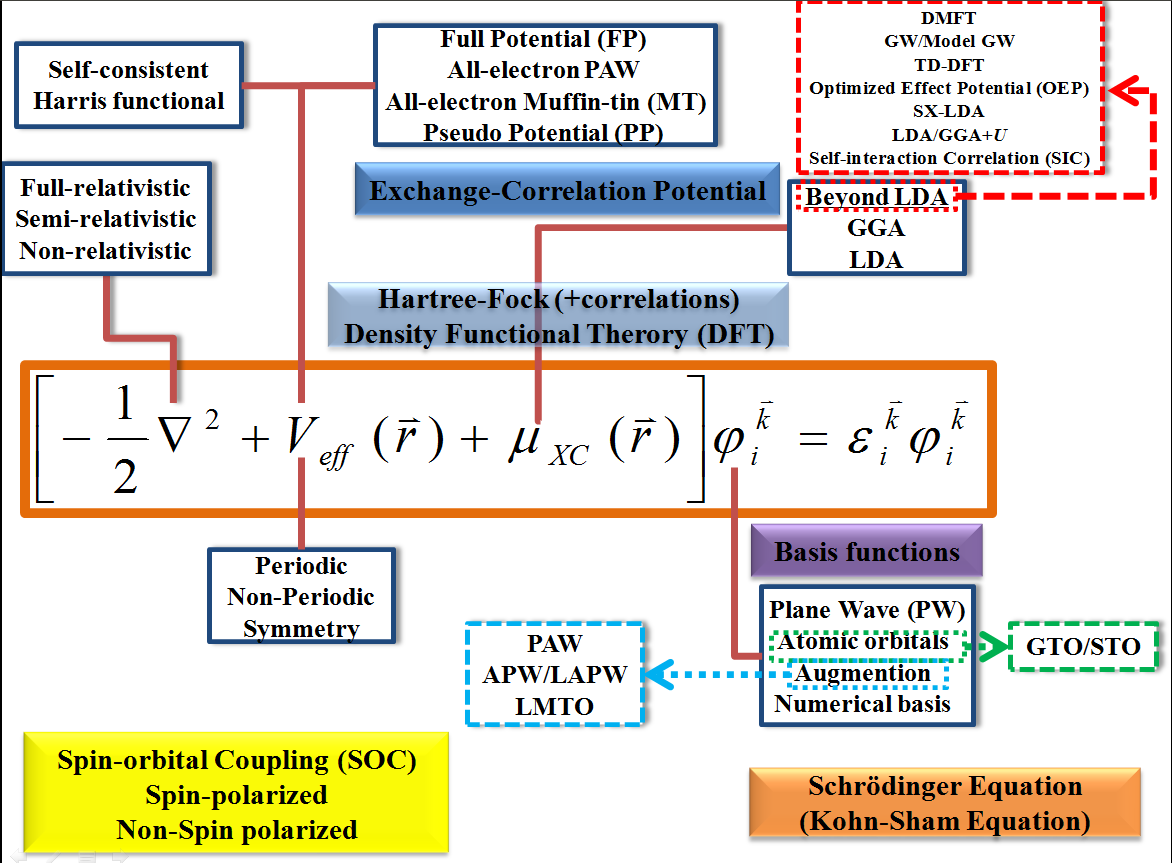
\includegraphics[width=0.5in, height=0.4in,viewport=0 0 1172 863,clip]{Figures/DFT.png}};
%  \node [box,below=0.5 of potential] (hamiltonian) {$\hat{H}_{KS}=-\frac{\hbar^2}{2m}\vec{\nabla}^2 + v_{\text{ext},s}(\vec r)$};
%  \node [box,below=0.5 of hamiltonian] (se) {$\hat{H}_{KS} \phi_i(\vec r)= E_i \phi_i(\vec r)$};
%  \node [box,below=0.5 of se] (density) {$\rho(\vec r)=\sum_{i=1}^n f_i\,|\phi_i(\vec r_i)|^2$};
%  \node [box,below=0.5 of density] (criterion) {Convergence criterion satisfied?};

%  \node [box,above=1.5 of potential, fill=orange!30, text width=20em] (initial) {Supply initial density guess $\rho_\text{ini}(\vec r)$ to Kohn Sham equations};
%  \node [box,below=1.5 of criterion, fill=blue!30, text width=20em] (energy) {Use $\rho_\text{fin}(\vec r)$ to minimize total energy functional $E_{V_\text{ext}}[\rho]=T_{e,s}[\phi_i\{\rho\}] + V_{ee,H}[\rho] + E_{xc}[\rho] + V_{eI}[\rho]$};

%  \path [arrow] (initial) -- (potential);
  \path [arrow] (Method) -- (Softwares);
  \path [arrow] (Theory) -- (Method);
  \path [arrow] (Basic-Equ) -- (Theory);
%  \path [arrow] (density) -- (criterion);

  \path [arrow] (PDE) -- (Algorithm);
  \path [arrow] (OS) -- (coding);
 % \path [arrow] (OS) -- (Figure);
  \path [arrow] (coding) |- (Softwares.east);
  \path [arrow] (Algorithm) |- (Softwares.west);
  \path [arrow] (Method.east) -- (coding.west);
  \path [arrow] (Method.west) -- (Algorithm.east);

%%%%%% ------------ 定义 虚线方框转角 -----------------  %%%%%%
%  \path
%  (potential.north west) ++(-1em,1em) coordinate (potential fit)
%  (criterion.south east) ++(1em,-1em) coordinate (criterion fit);

%%%%%% ------------ 绘制 虚线方框 -----------------  %%%%%%
%  \node [rectangle,draw,dashed,inner sep=1em,fit=(potential fit) (criterion fit)] (enclosure) {};
%  \node [above=-0.8em of enclosure,anchor=south,draw,outer sep=0pt,fill=white] (enclosure label) {\Large\textbf{Kohn-Sham method}};

%  \path [arrow] (criterion) -- (energy) node [midway,left=0.1,draw,outer sep=0pt,fill=white] (TextNode) {Yes};
%  \path [draw,thick] (criterion.south) ++(0em,-1em) -- (criterion fit) node [midway,below=0.1,sloped,draw,outer sep=0pt,fill=white] (TextNode) {No};
%  \draw [arrow] (criterion fit) |- (potential.east);
\end{tikzpicture}
}

\frame
{
	\frametitle{\textrm{DFT-SCF}}
\begin{figure}[h!]
\centering
\vspace*{-0.25in}
\hspace*{-0.80in}
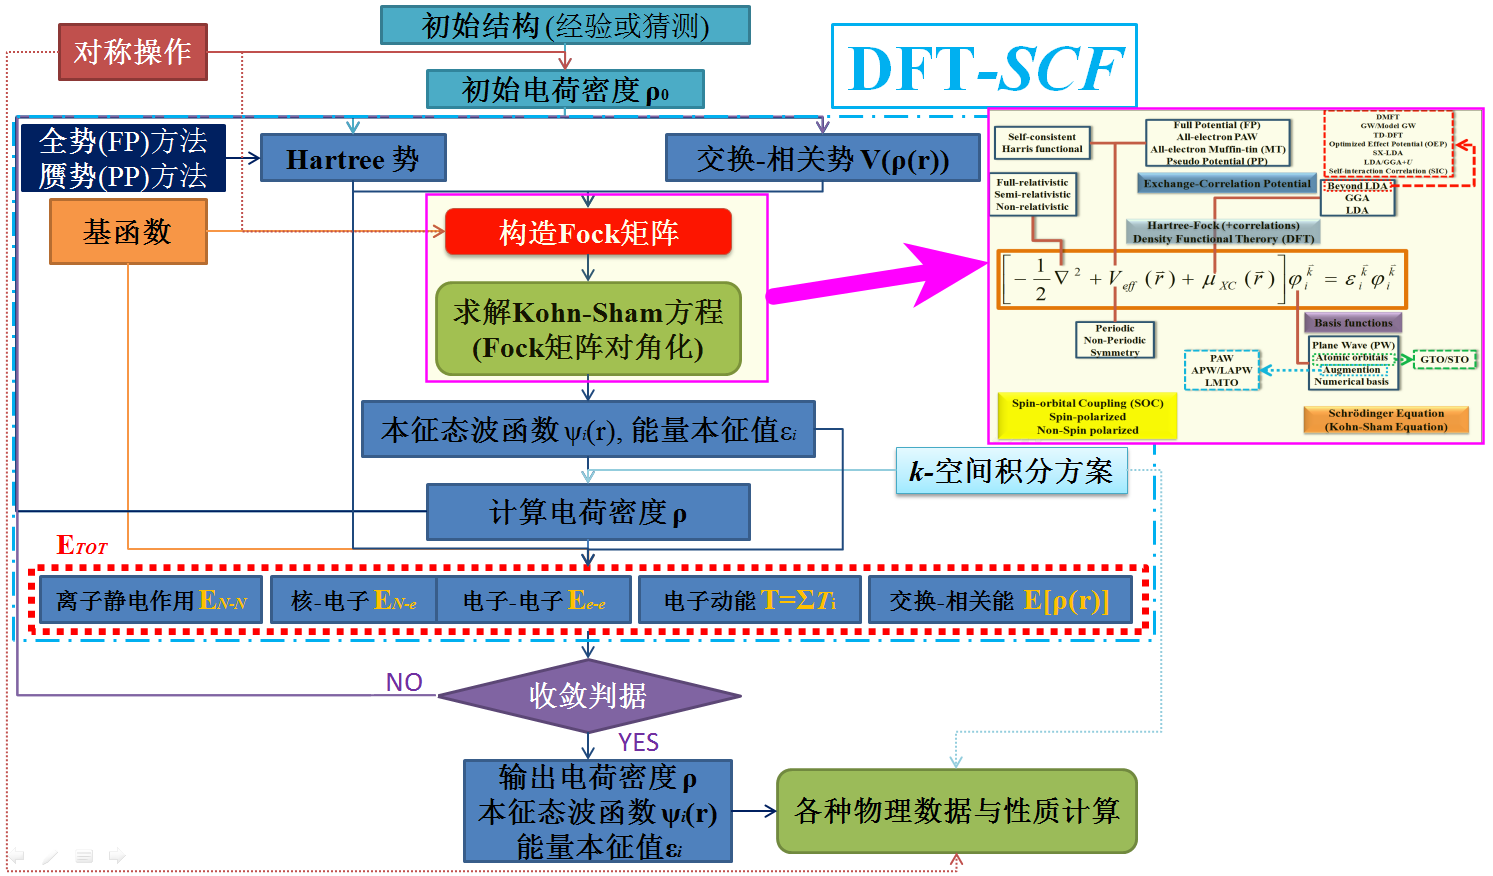
\includegraphics[height=2.80in,width=4.95in,viewport=5 3 1490 870,clip]{Figures/DFT-SCF_2.png}
%\caption{\tiny \textrm{Pseudopotential for metallic sodium, based on the empty core model and screened by the Thomas-Fermi dielectric function.}}%(与文献\cite{EPJB33-47_2003}图1对比)
\label{DFT-SCF-2}
\end{figure}
}

\frame
{
	\frametitle{密度泛函与粒子表示表示}
\begin{figure}[h!]
\vskip -10pt
\centering
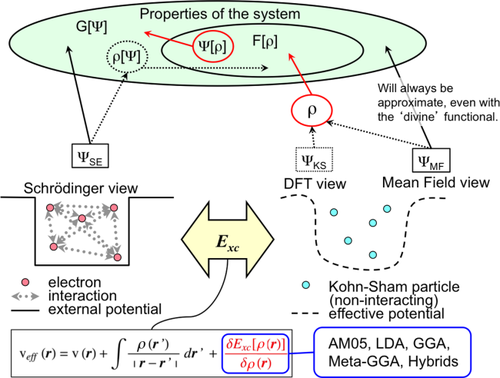
\includegraphics[height=2.65in,width=3.8in,viewport=0 0 362 275,clip]{Figures/DFT-particle-density.png}
\caption{\fontsize{6.0pt}{4.5pt}\selectfont{\textrm{Properties of a quantum mechanical system can be calculated by solving the SE (left). A more tractable, formally equivalent way is to solve the DFT KS equations (right).}}}%(与文献\cite{EPJB33-47_2003}图1对比)
\label{Schrodinger-equation-vs-Kohn-Sham-equation}
\end{figure}
}

\frame
{
	\frametitle{材料计算软件发展现状}
\begin{figure}[h!]
\vspace*{-0.16in}
\centering
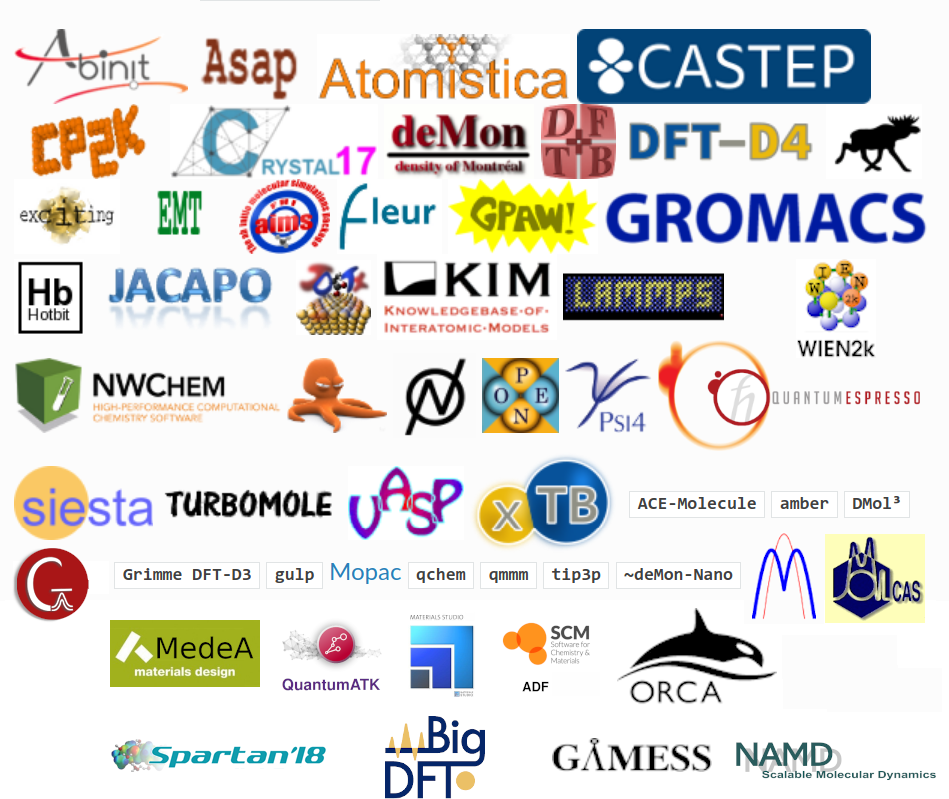
\includegraphics[width=3.30in]{Figures/Softwares_logo.png}
%\caption{\tiny \textrm{Pseudopotential for metallic sodium, based on the empty core model and screened by the Thomas-Fermi dielectric function.}}%(与文献\cite{EPJB33-47_2003}图1对比)
\label{Softwares}
\end{figure}
}

\frame
{
	\frametitle{国产第一原理计算软件现状}
\begin{figure}[h!]
\vspace*{-0.19in}
\centering
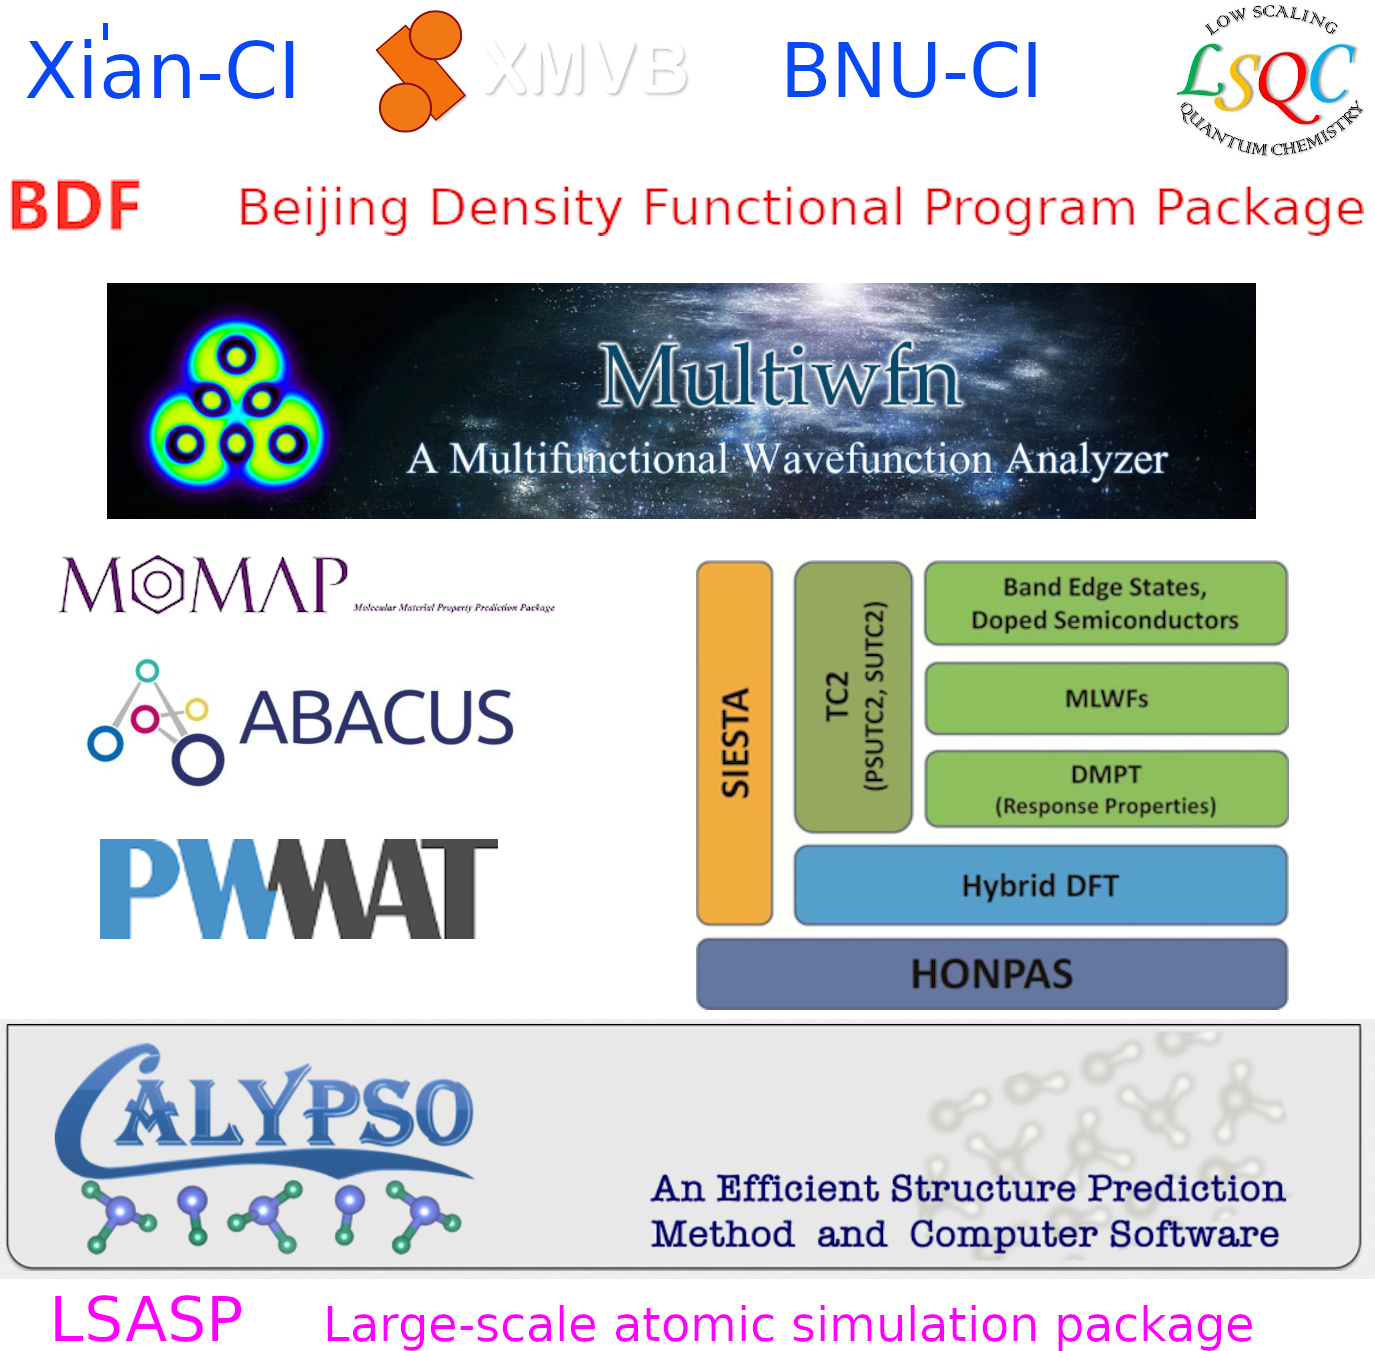
\includegraphics[width=2.83in]{Figures/Softwares_China-logo.png}
%\caption{\tiny \textrm{Pseudopotential for metallic sodium, based on the empty core model and screened by the Thomas-Fermi dielectric function.}}%(与文献\cite{EPJB33-47_2003}图1对比)
\label{Software-China}
\end{figure}
	\fontsize{6.2pt}{5.2pt}\selectfont{\textcolor{red}{中国学科发展战略\,$\cdot$\,理论与计算化学,~~国家自然科学基金委员会,~中国科学院,~~北京:~科学出版社,~~2016}}
}

\frame
{
	\frametitle{\textrm{VASP}软件简介}
	\textrm{VASP}软件是维也纳大学\textrm{(Universit\"at Wien)}~\textrm{G. Kresse}等开发的第一原理模拟软件包
	\begin{itemize}
		\item \textrm{VASP}采用\textrm{PAW~(Projector Augmented-Wave)}方法\upcite{PRB50-17953_1994,PRB59-1758_1999},平衡了赝势方法和全电子计算优点,兼顾了计算的精度和效率
		\item \textrm{VASP}在实空间优化投影函数\textrm{(Projector)},将主要的计算过程变换到实空间完成,大大节省了内存的开销%,保证了计算精度和效率
		\item \textrm{VASP}通过引入多样的优化算法,提高了矩阵对角化和电荷密度搜索的效率%\upcite{CMS6-15_1996,PRB54-11169_1996}
		\item 在\textrm{VASP}的并行计算中,有效均衡了各节点处理\textrm{FFT}变换负载和通信,提升了软件的并行效率
	\end{itemize}
	相比于其他第一原理计算软件,\textrm{VASP}从物理思想与方法、优化算法和并行计算实现等多个方面都有更为出色的性能%\upcite{PRL55-2471_1985,PRB47-10142_1993}
}

%\frame
%{
%	\frametitle{\textrm{VASP}的开发团队}
%\begin{figure}[h!]
%\centering
%\vspace*{-0.25in}
%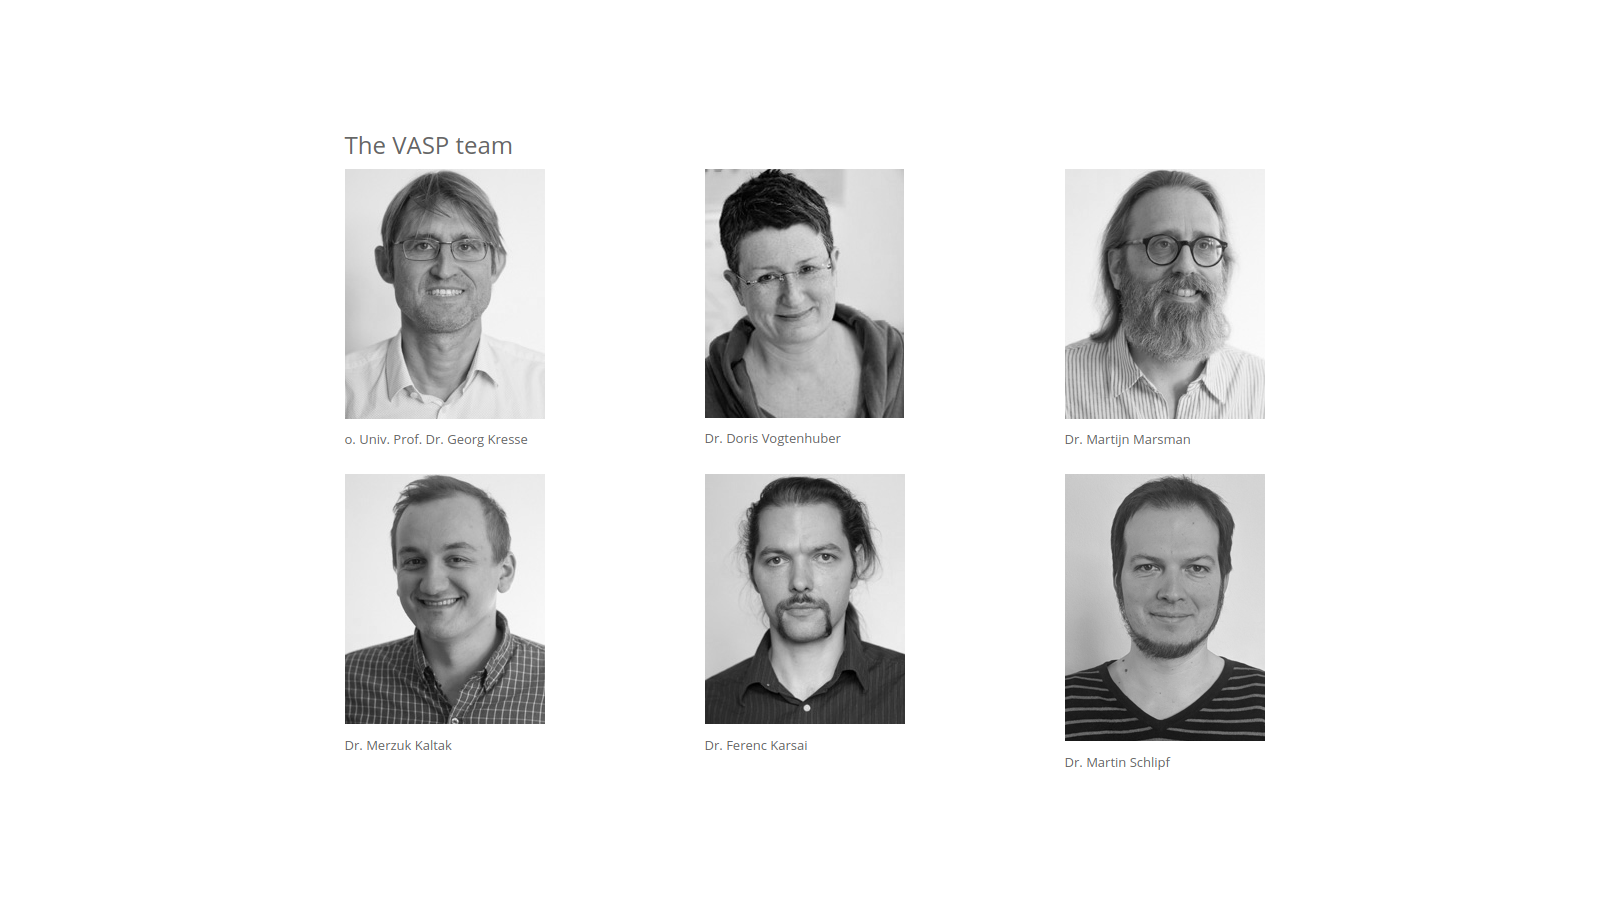
\includegraphics[height=2.70in,width=4.05in,viewport=330 130 1280 770,clip]{Figures/VASP_team.png}
%\caption{\tiny \textrm{The development team of VASP.}}%(与文献\cite{EPJB33-47_2003}图1对比)
%\label{VASP_team}
%\end{figure}
%}
%
%\begin{frame}[allowframebreaks]{\textrm{VASP}的主程序结构}
%\begin{figure}[h!]
%\vskip -10pt
%\centering
%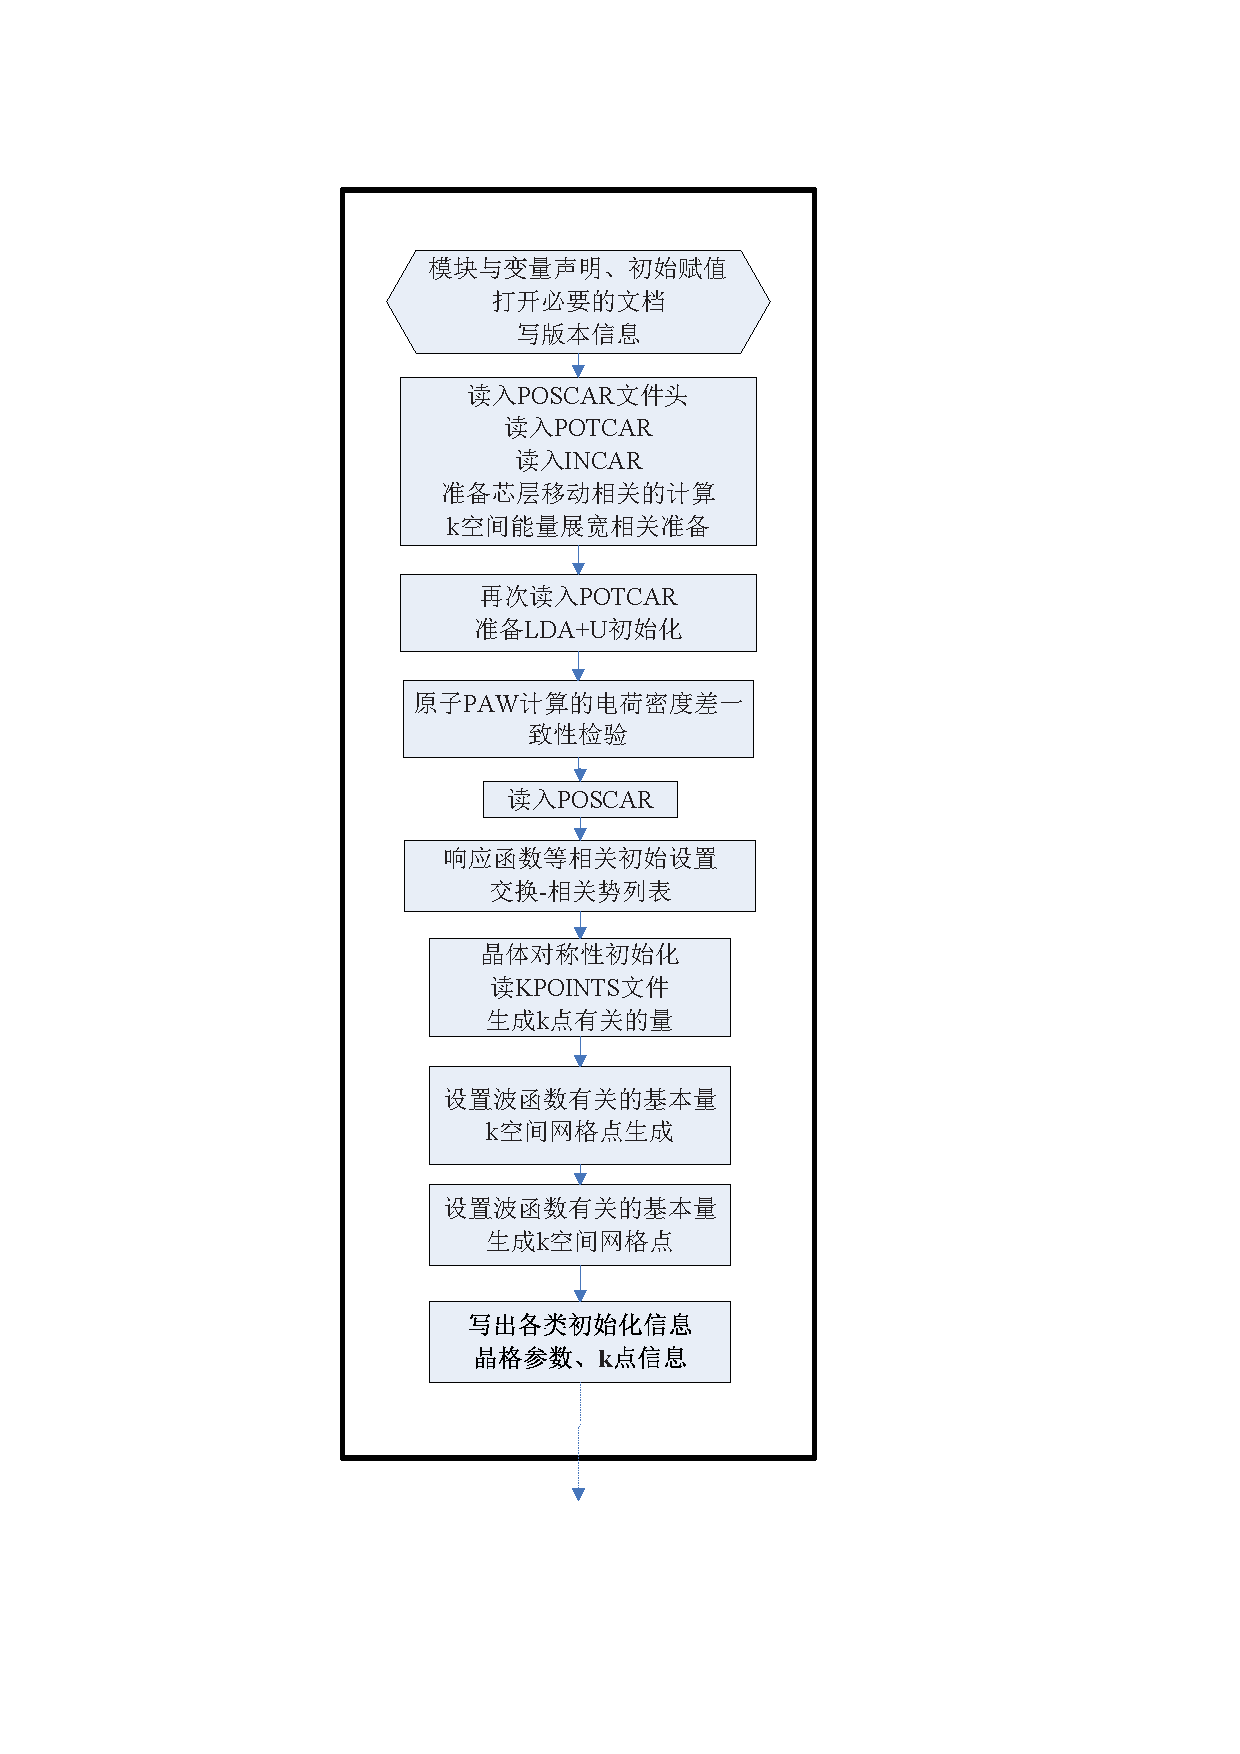
\includegraphics[height=2.65in,width=4.0in,viewport=0 360 562 720,clip]{Figures/VASP_main_Flow-1.png}
%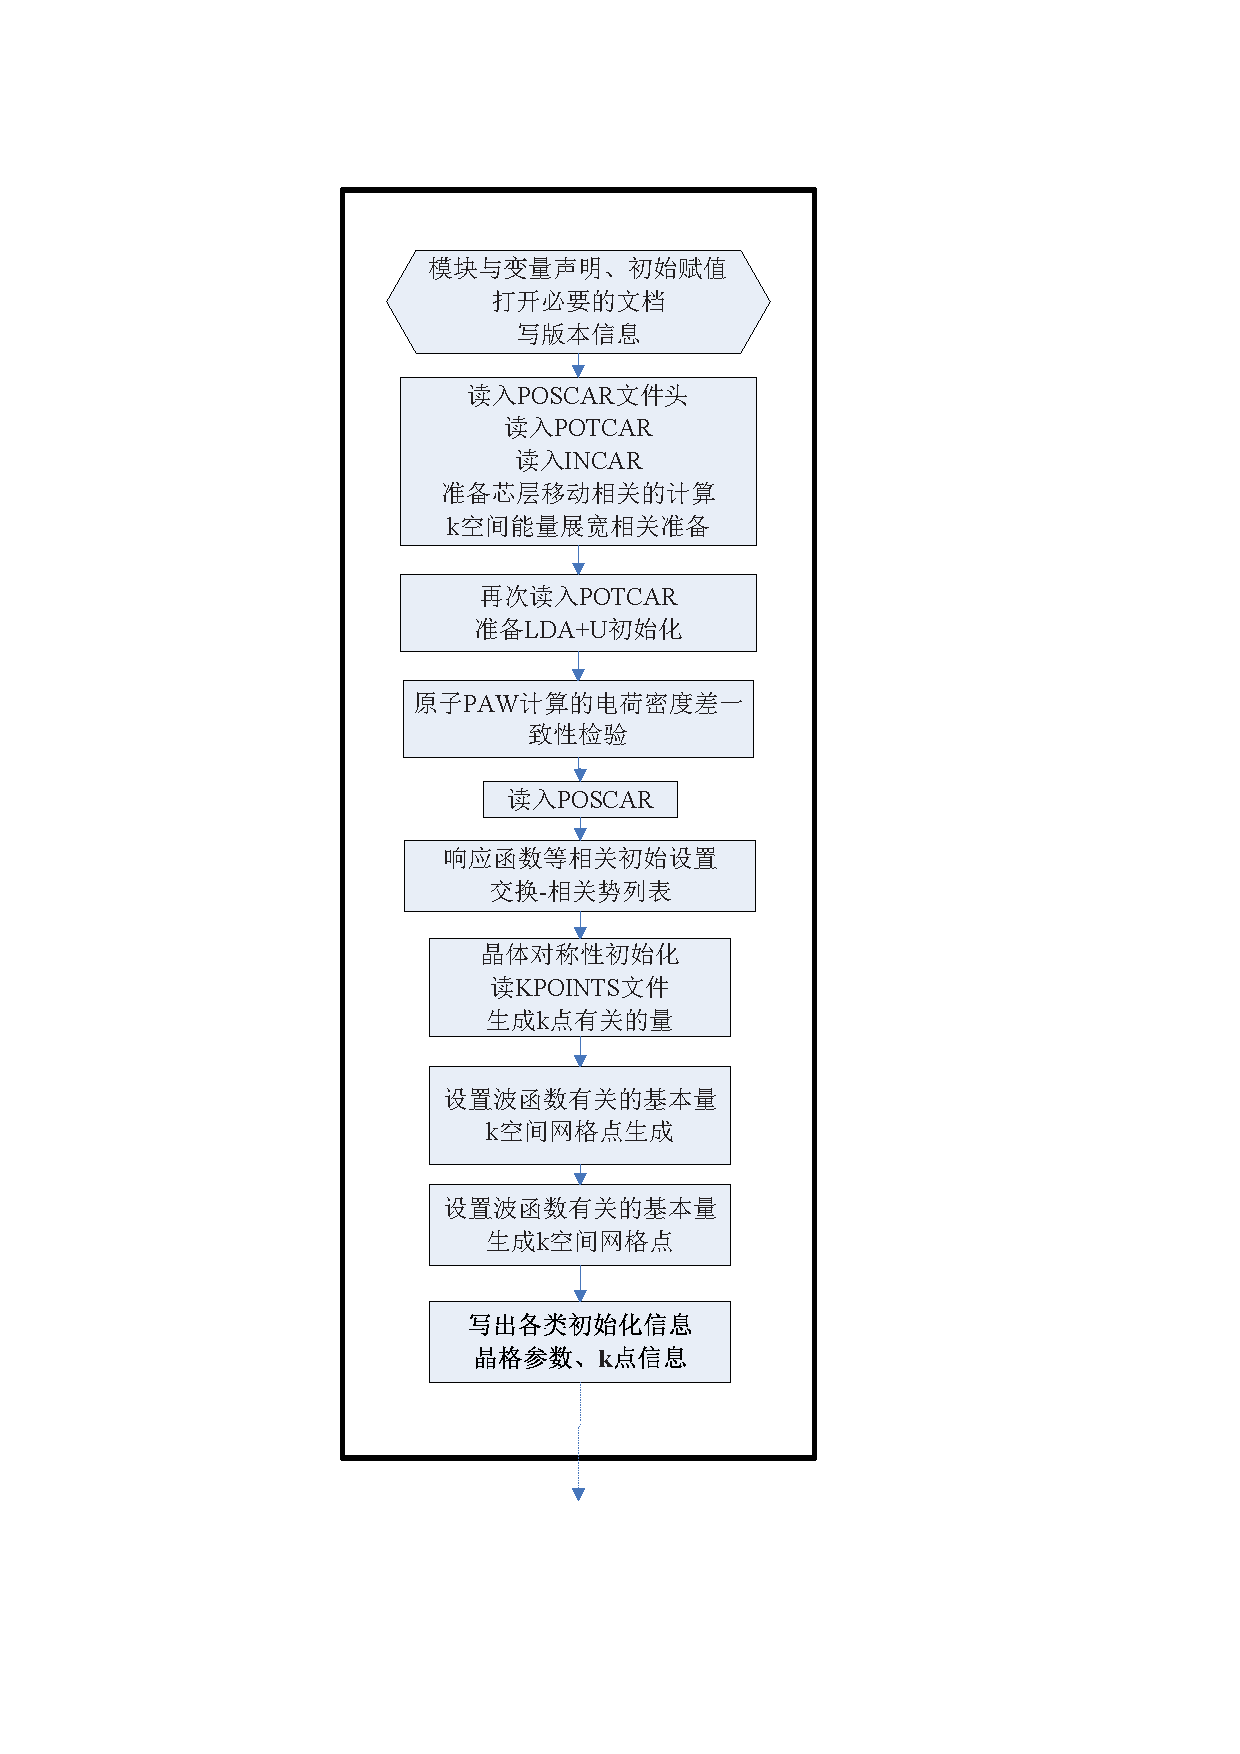
\includegraphics[height=2.65in,width=4.0in,viewport=0 0 562 360,clip]{Figures/VASP_main_Flow-1.png}
%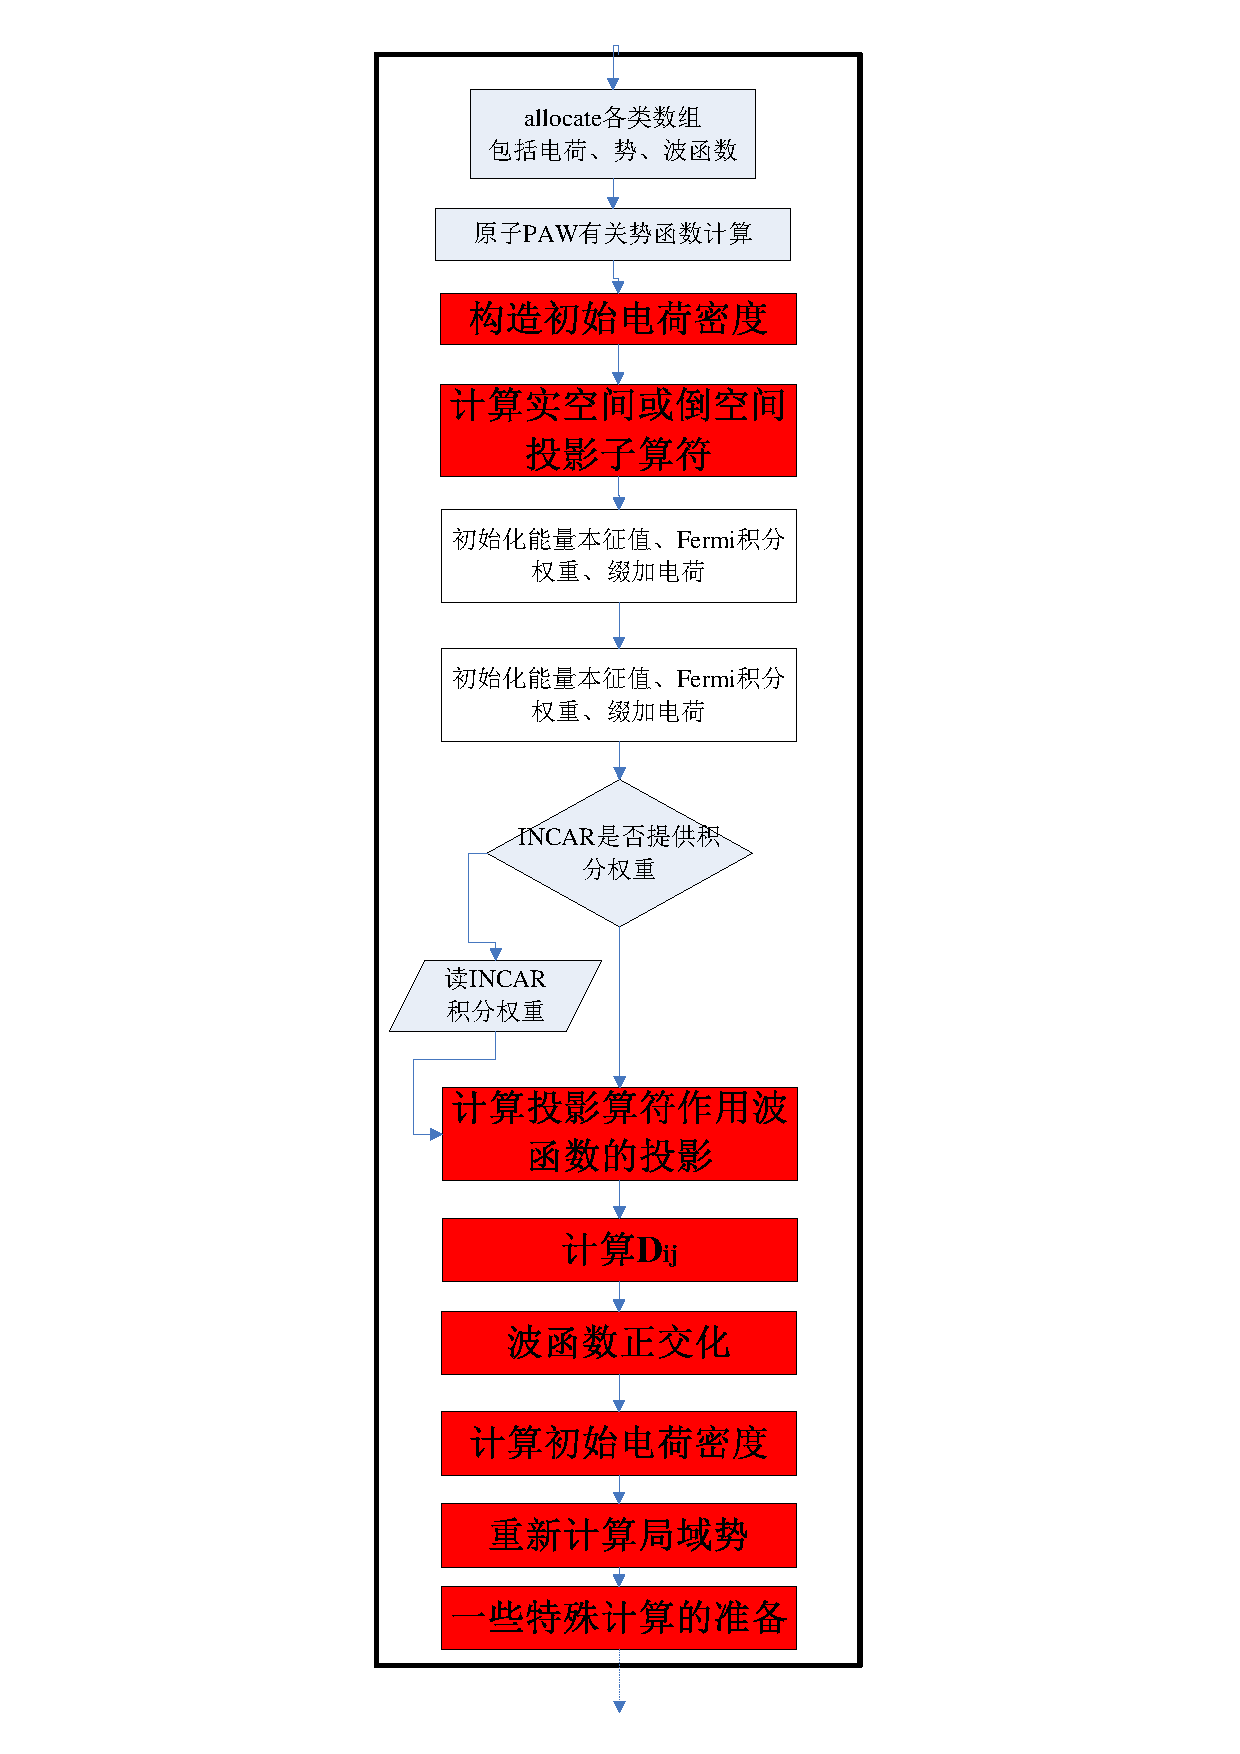
\includegraphics[height=2.35in,width=4.0in,viewport=0 370 562 680,clip]{Figures/VASP_main_Flow-2.png}
%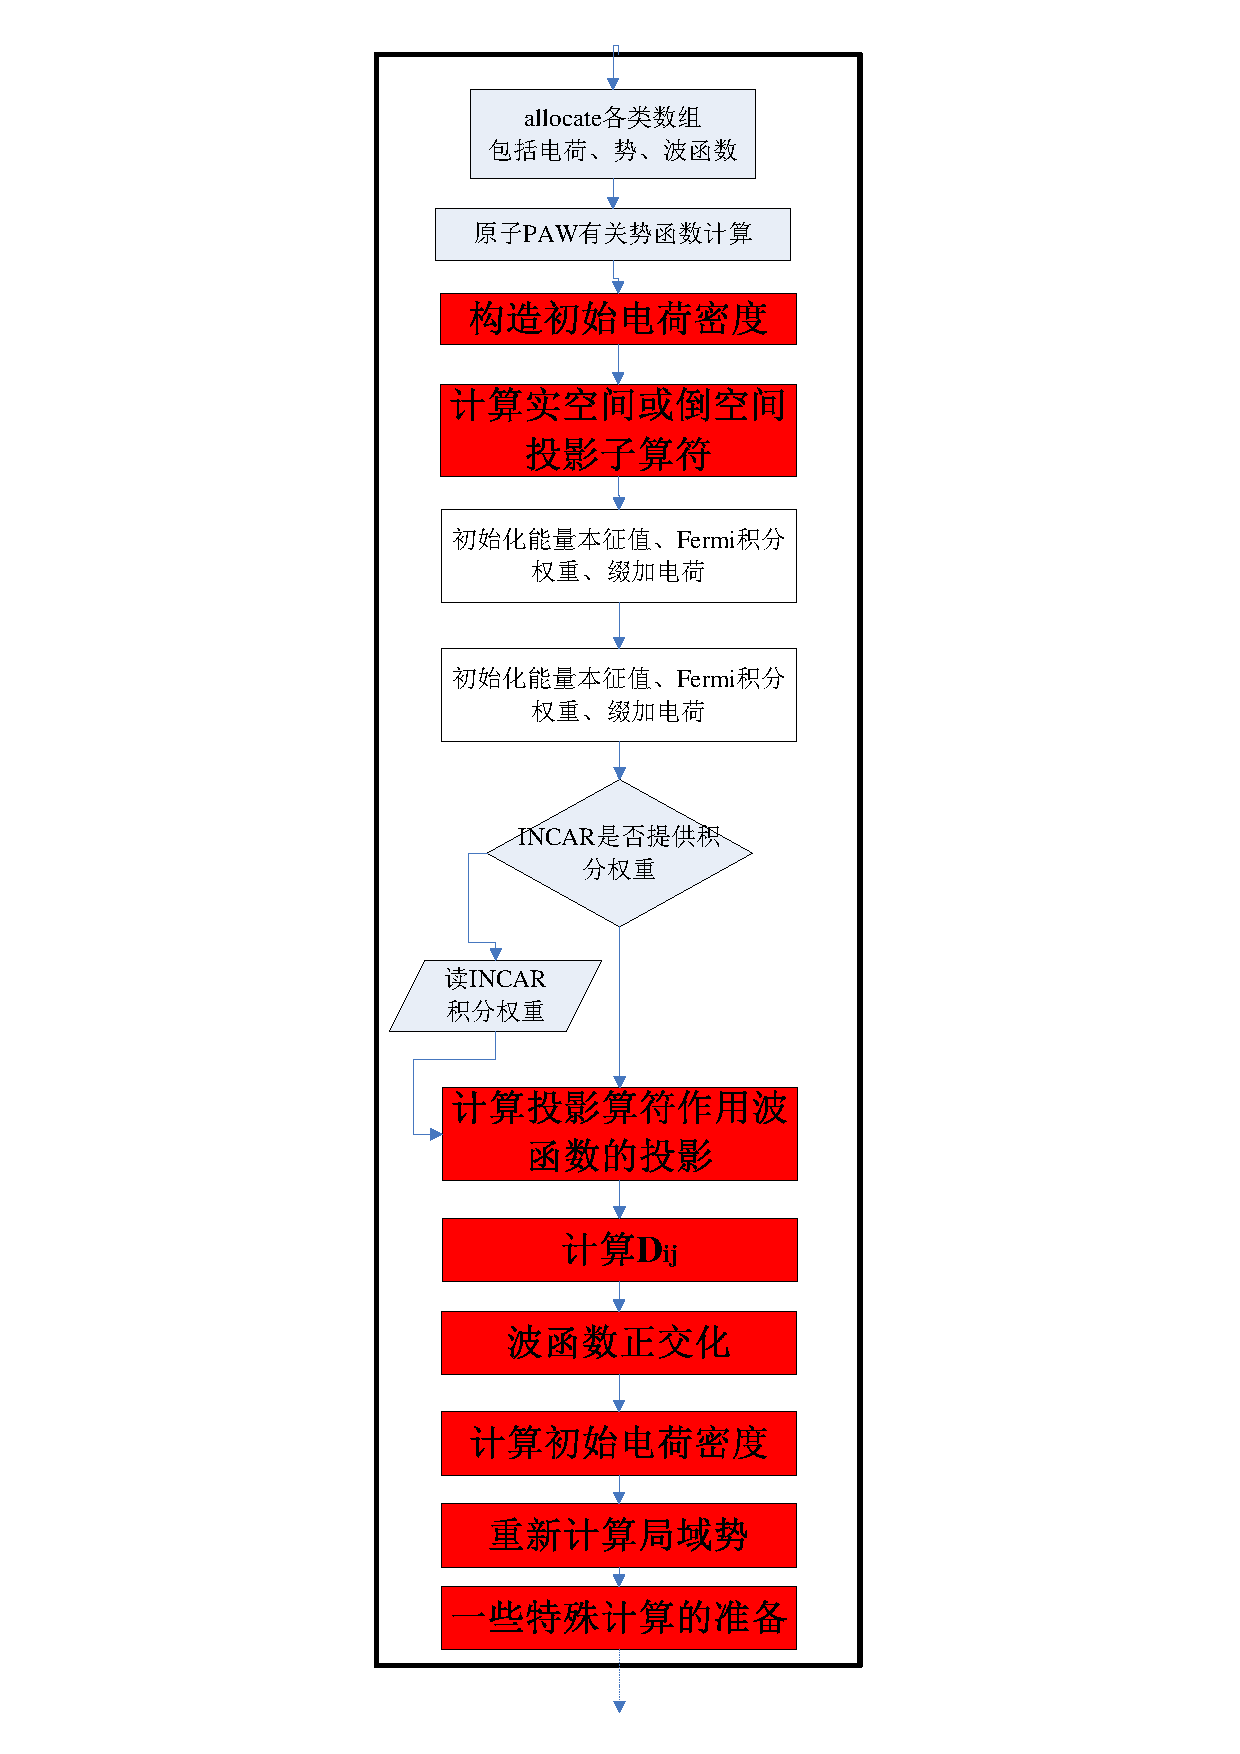
\includegraphics[height=2.50in,width=4.0in,viewport=0 0 562 370,clip]{Figures/VASP_main_Flow-2.png}
%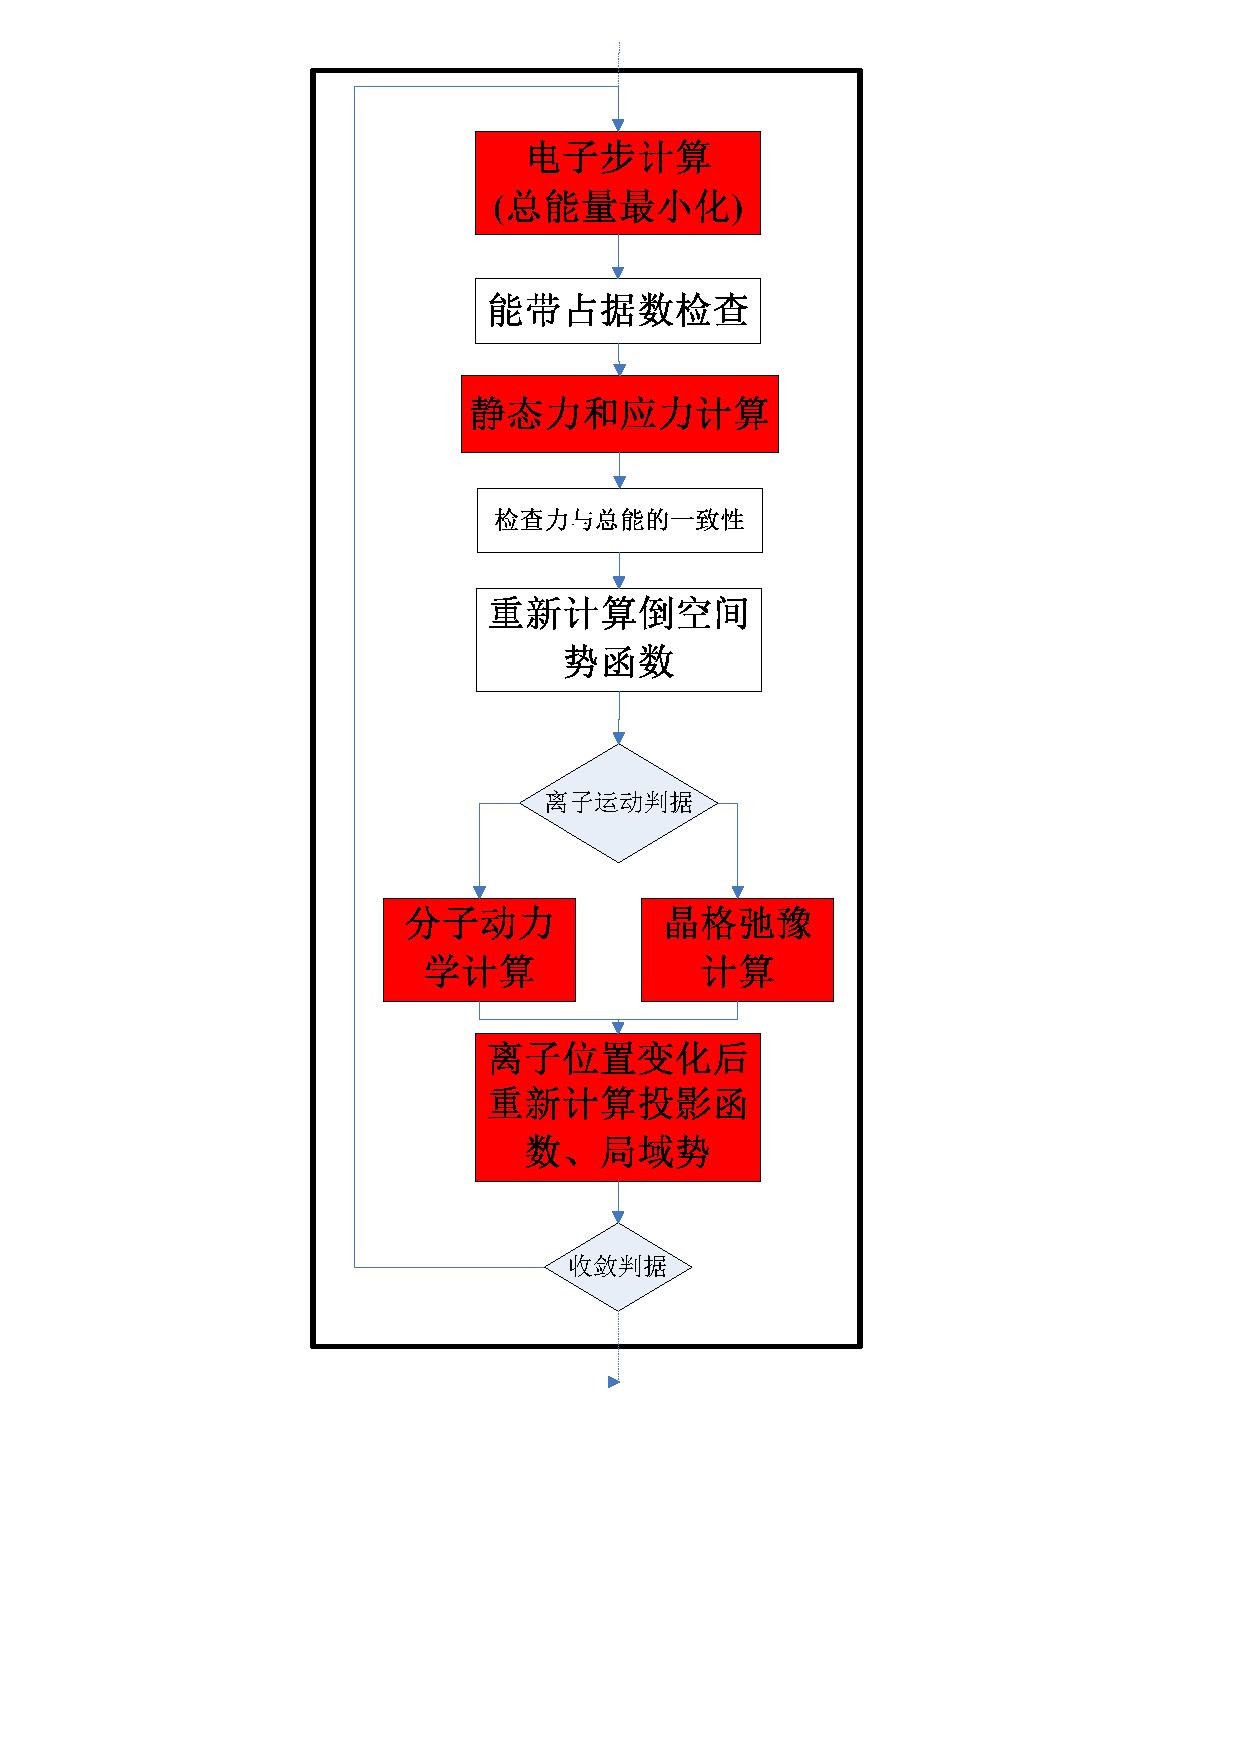
\includegraphics[height=2.45in,width=4.0in,viewport=0 350 562 660,clip]{Figures/VASP_main_Flow-3.png}
%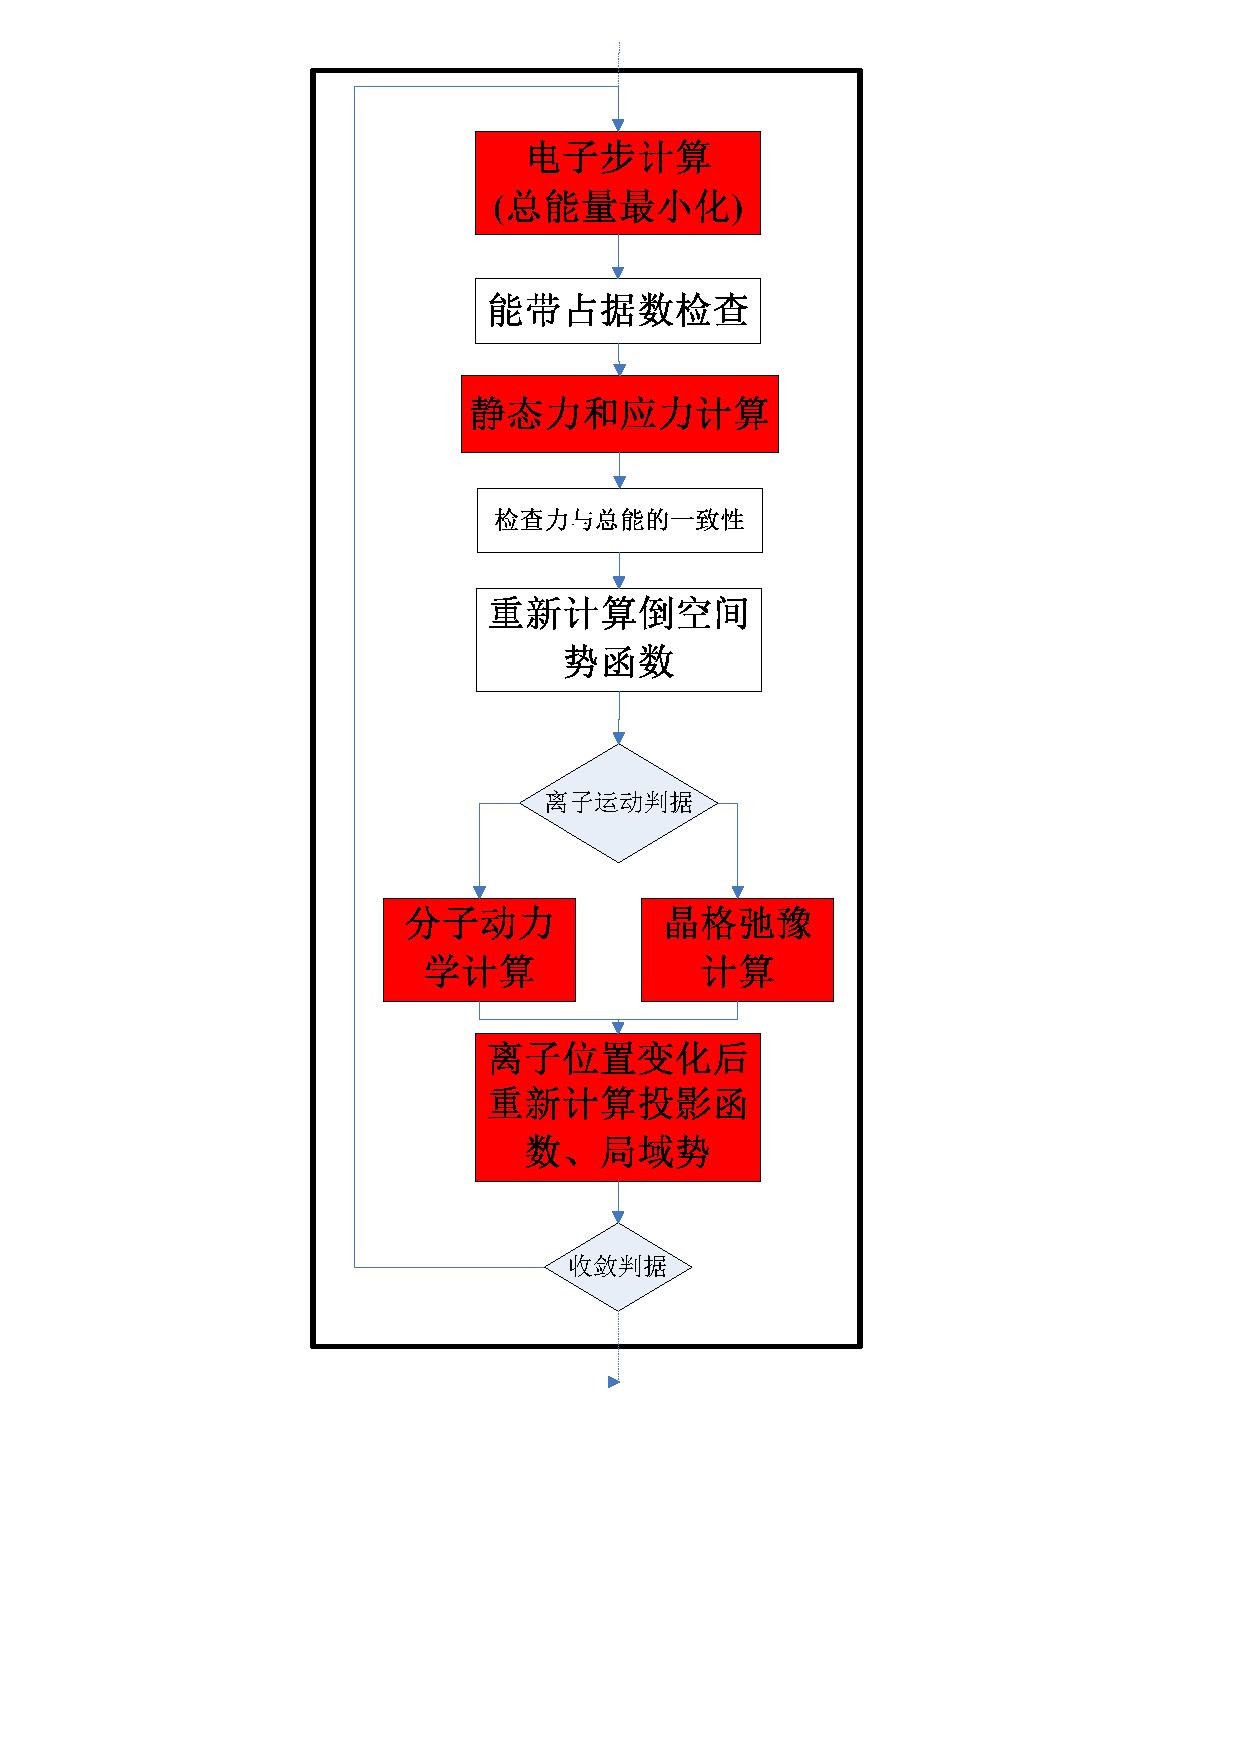
\includegraphics[height=2.50in,width=4.0in,viewport=0 0 562 350,clip]{Figures/VASP_main_Flow-3.png}
%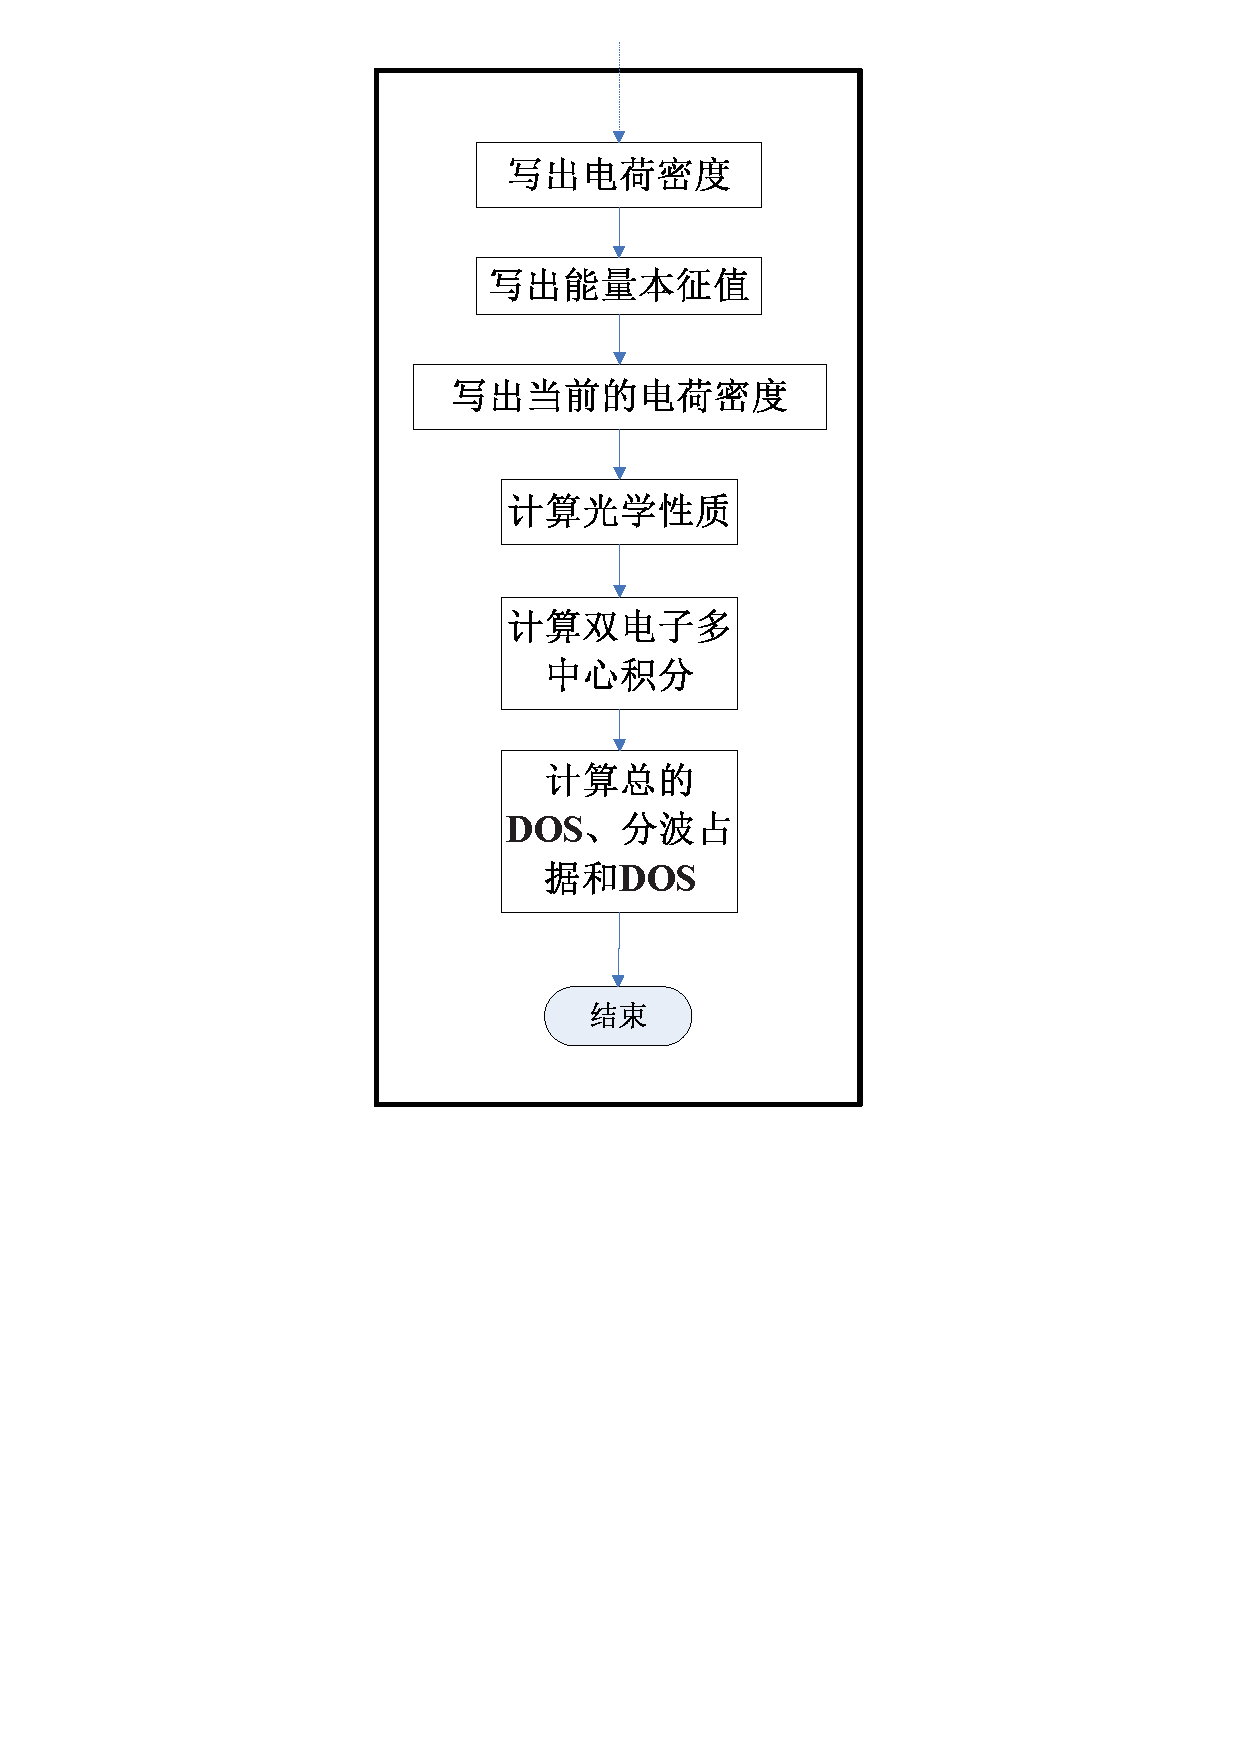
\includegraphics[height=2.30in,width=4.0in,viewport=0 215 562 530,clip]{Figures/VASP_main_Flow-4.png}
%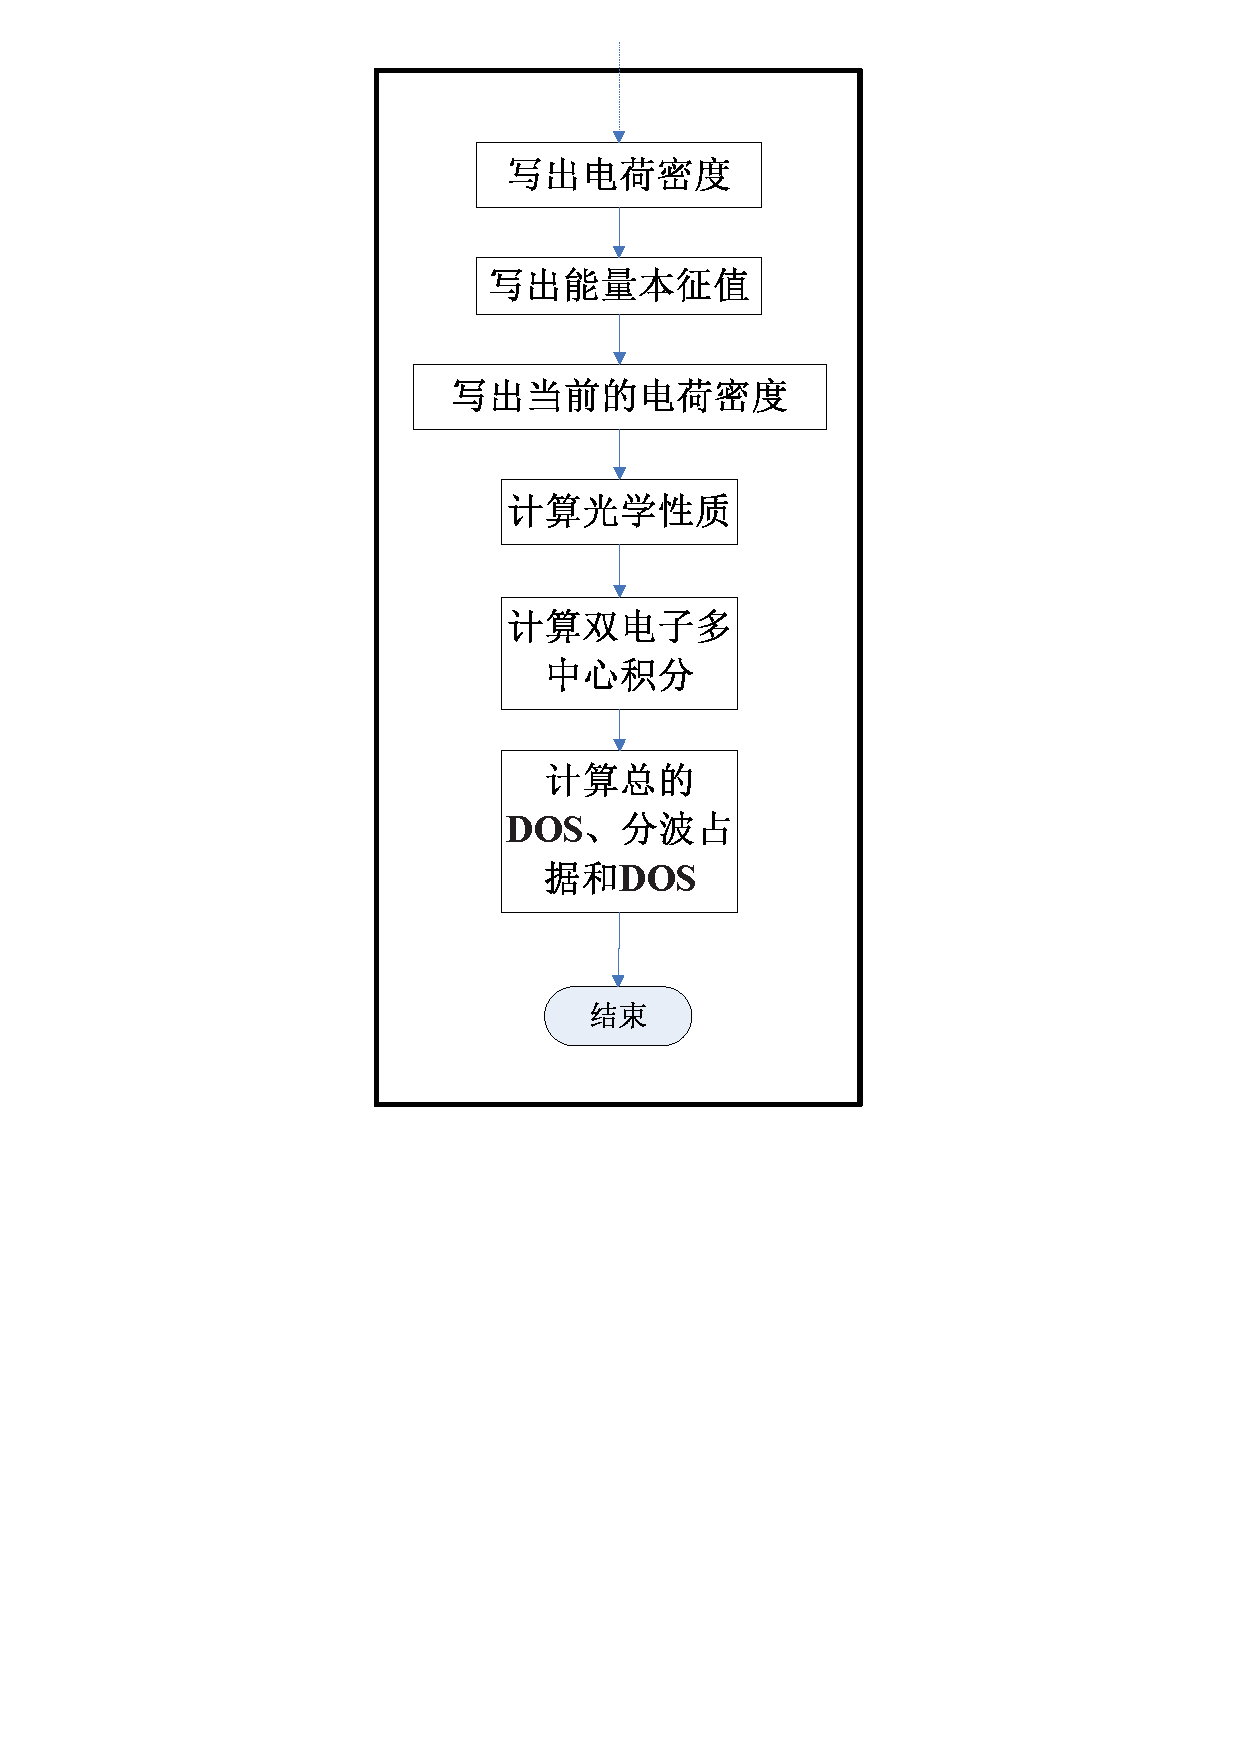
\includegraphics[height=1.40in,width=4.0in,viewport=0 0 562 215,clip]{Figures/VASP_main_Flow-4.png}
%\caption{\tiny \textrm{The Flow of main program for VASP.}}%(与文献\cite{EPJB33-47_2003}图1对比)
%\label{FLOW_of_VASP}
%\end{figure}
%\end{frame}
%
%\frame[allowframebreaks]
%{\frametitle{\textrm{VASP}运行分析}
%\begin{figure}[h!]
%	\vspace{-0.15in}
%\centering
%%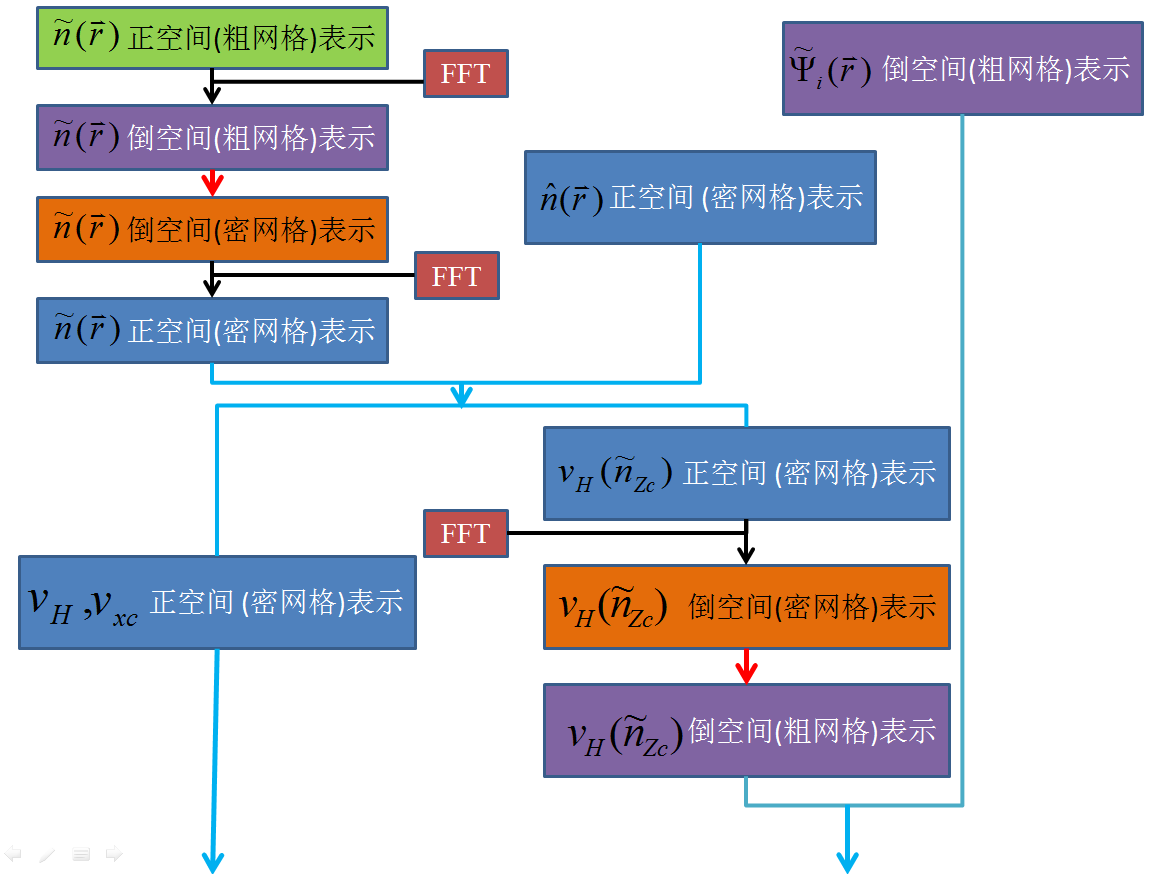
\includegraphics[height=2.7in,width=4.0in,viewport=0 0 1180 875,clip]{Figures/dual_grid.png}
%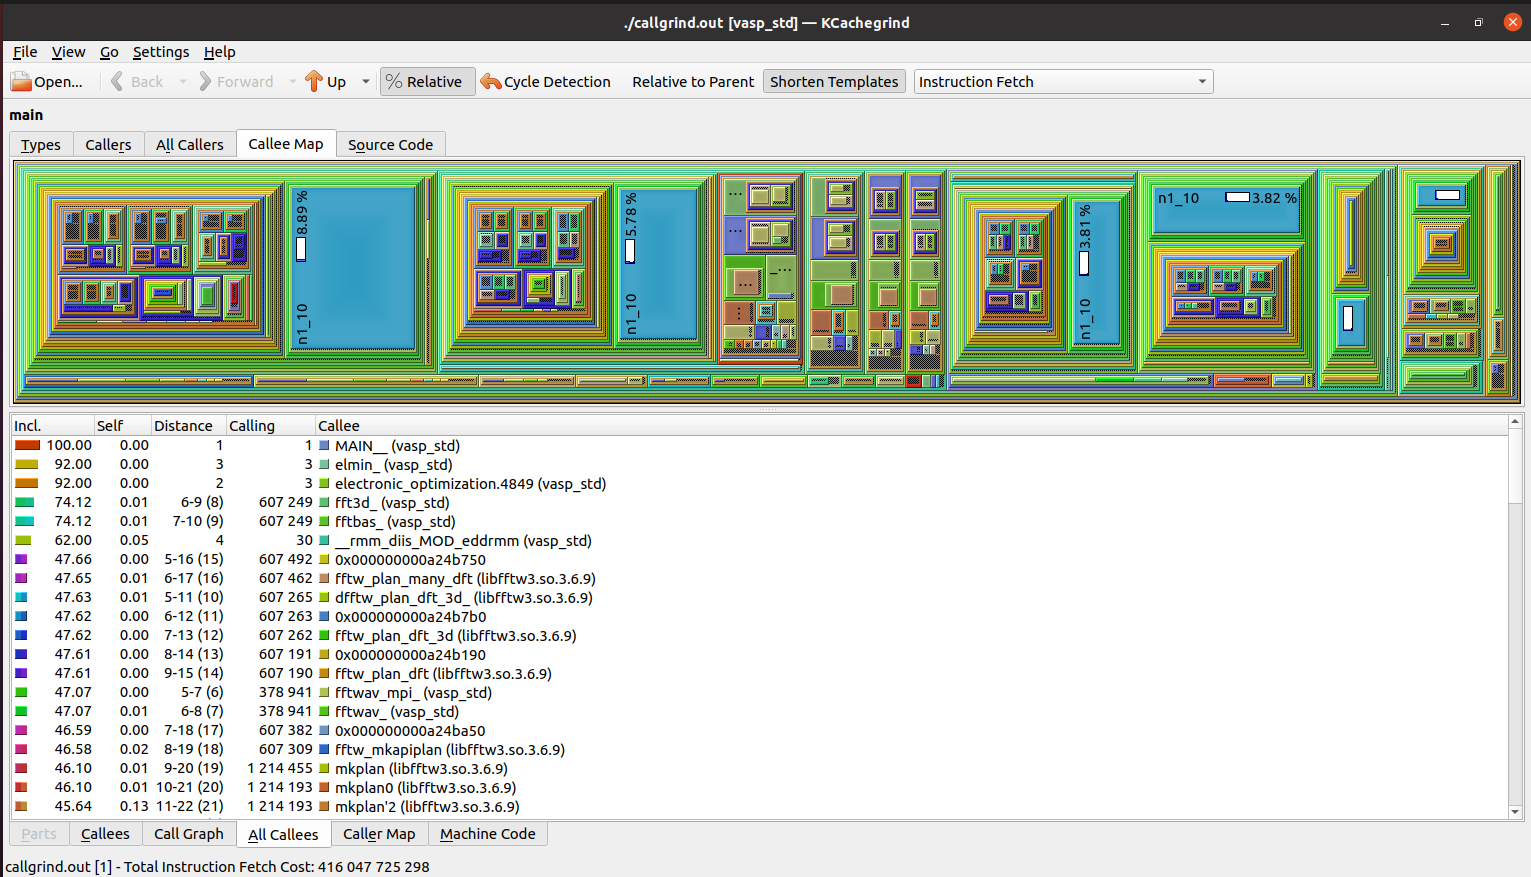
\includegraphics[height=2.5in,width=4.05in,viewport=0 0 1531 877,clip]{Figures/Kcachegrid_analyasis-VASP-01.png}
%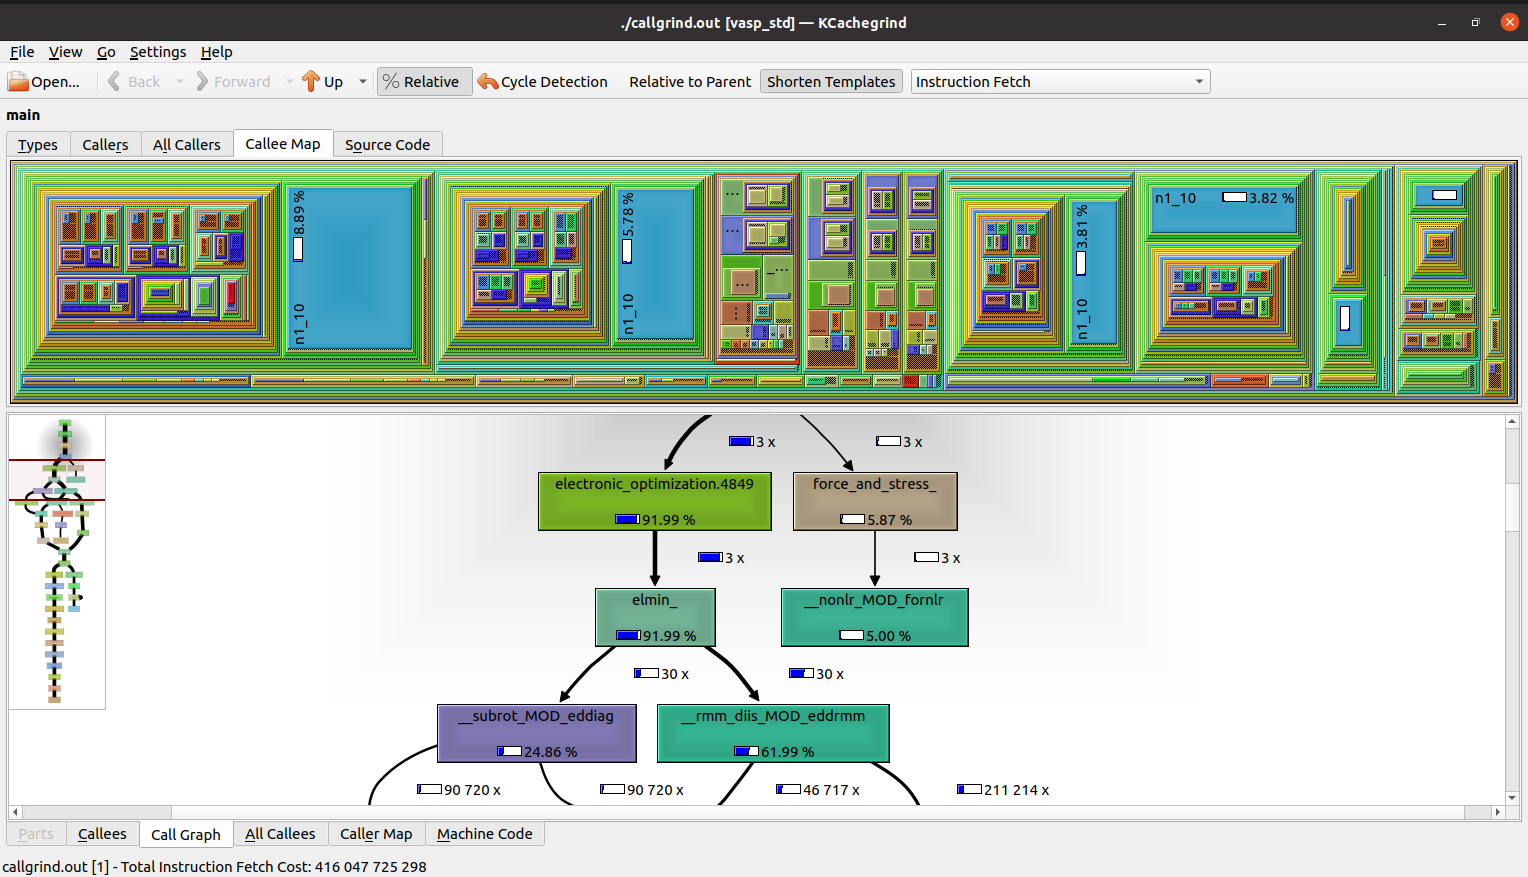
\includegraphics[height=2.5in,width=4.05in,viewport=0 0 1531 877,clip]{Figures/Kcachegrid_analyasis-VASP-02.png}
%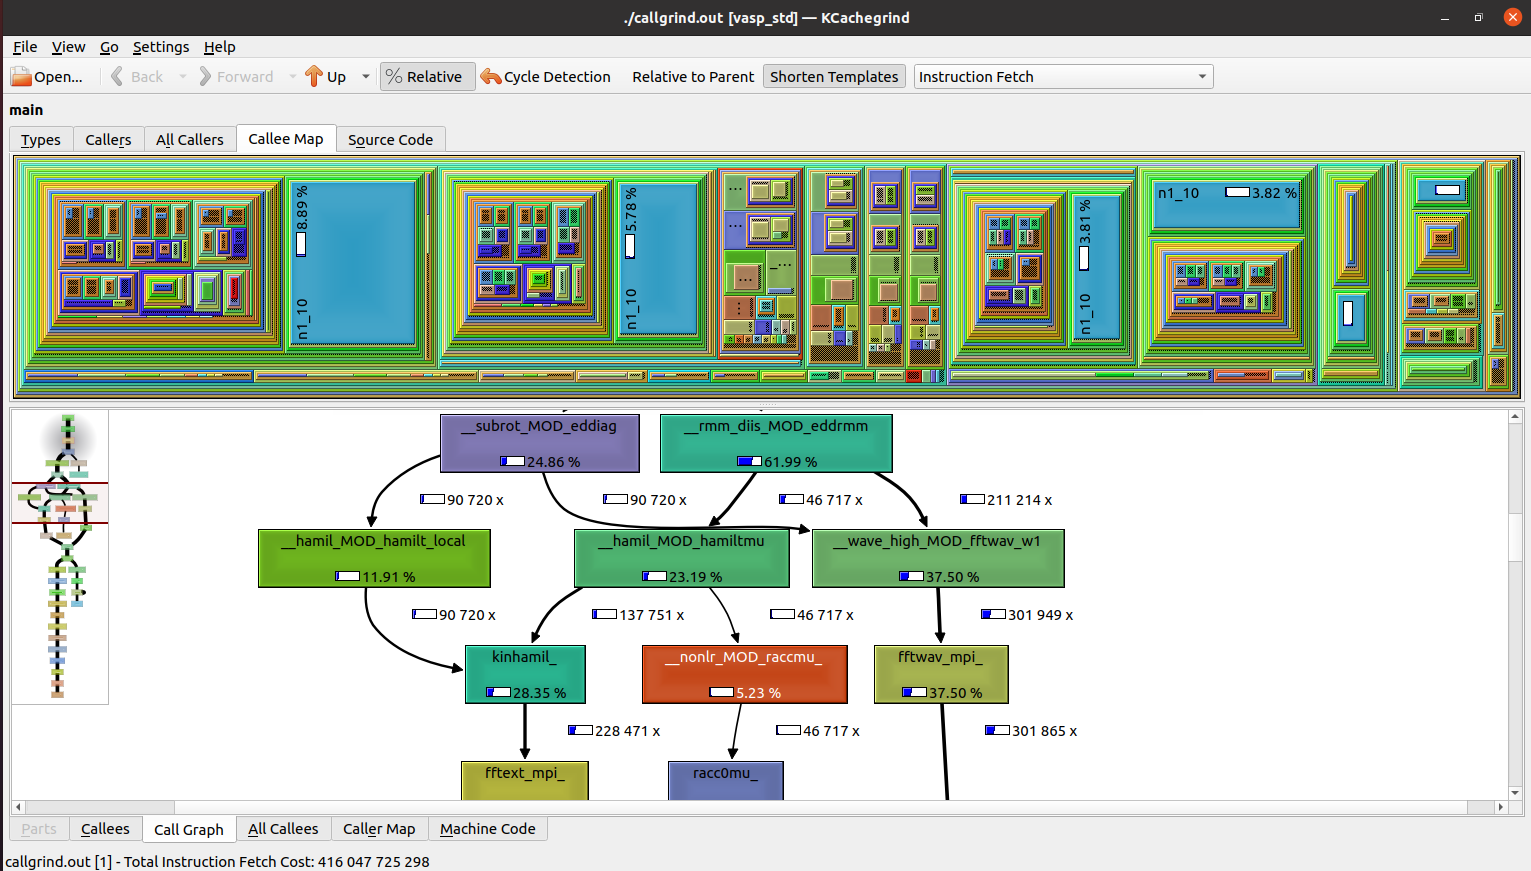
\includegraphics[height=2.5in,width=4.05in,viewport=0 0 1531 877,clip]{Figures/Kcachegrid_analyasis-VASP-03.png}
%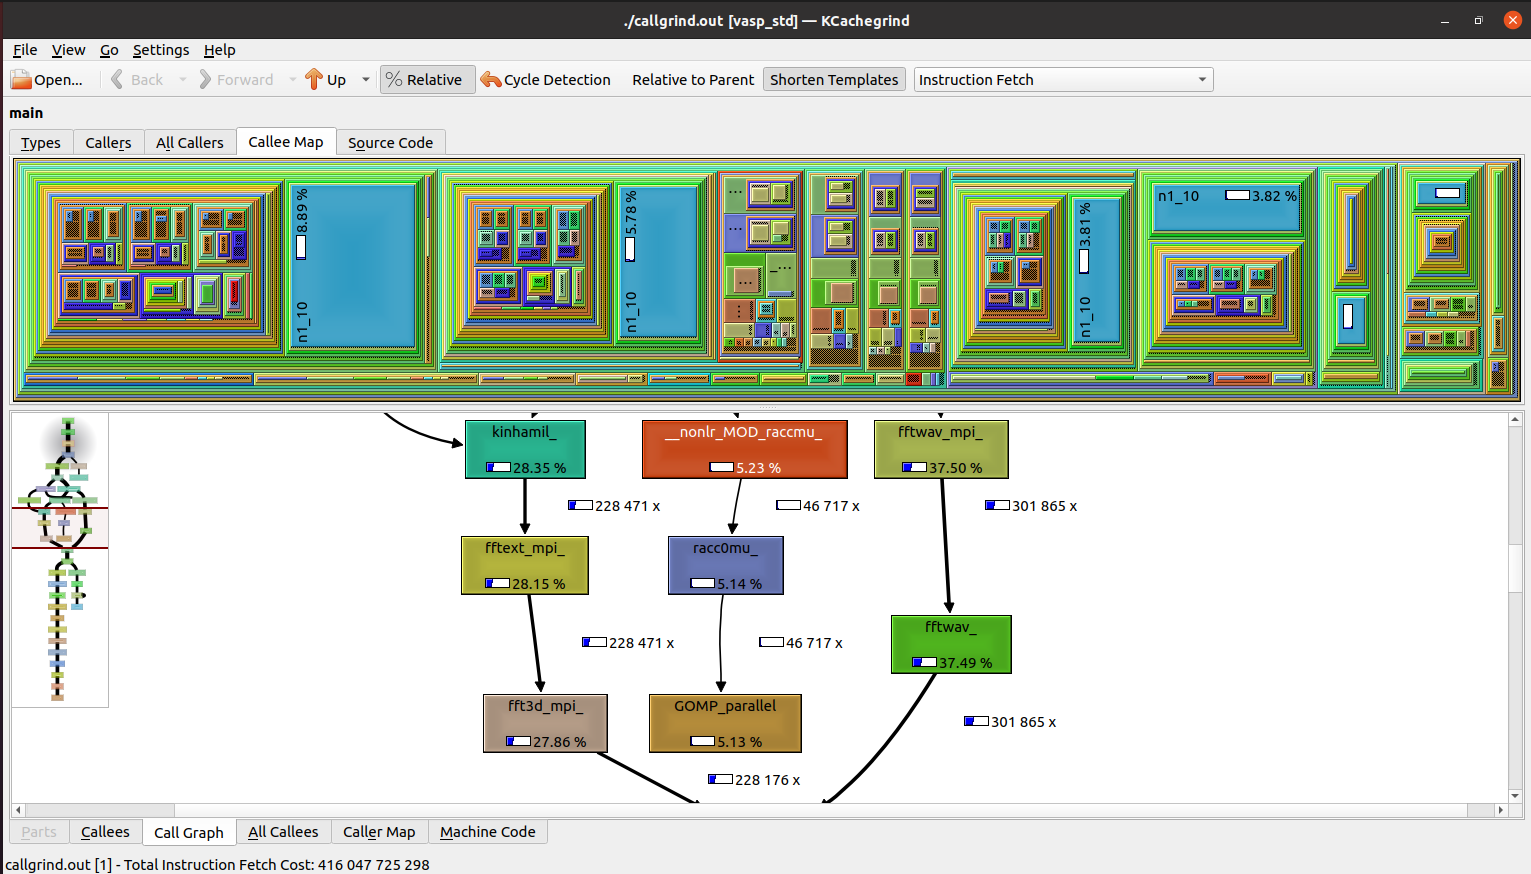
\includegraphics[height=2.5in,width=4.05in,viewport=0 0 1531 877,clip]{Figures/Kcachegrid_analyasis-VASP-04.png}
%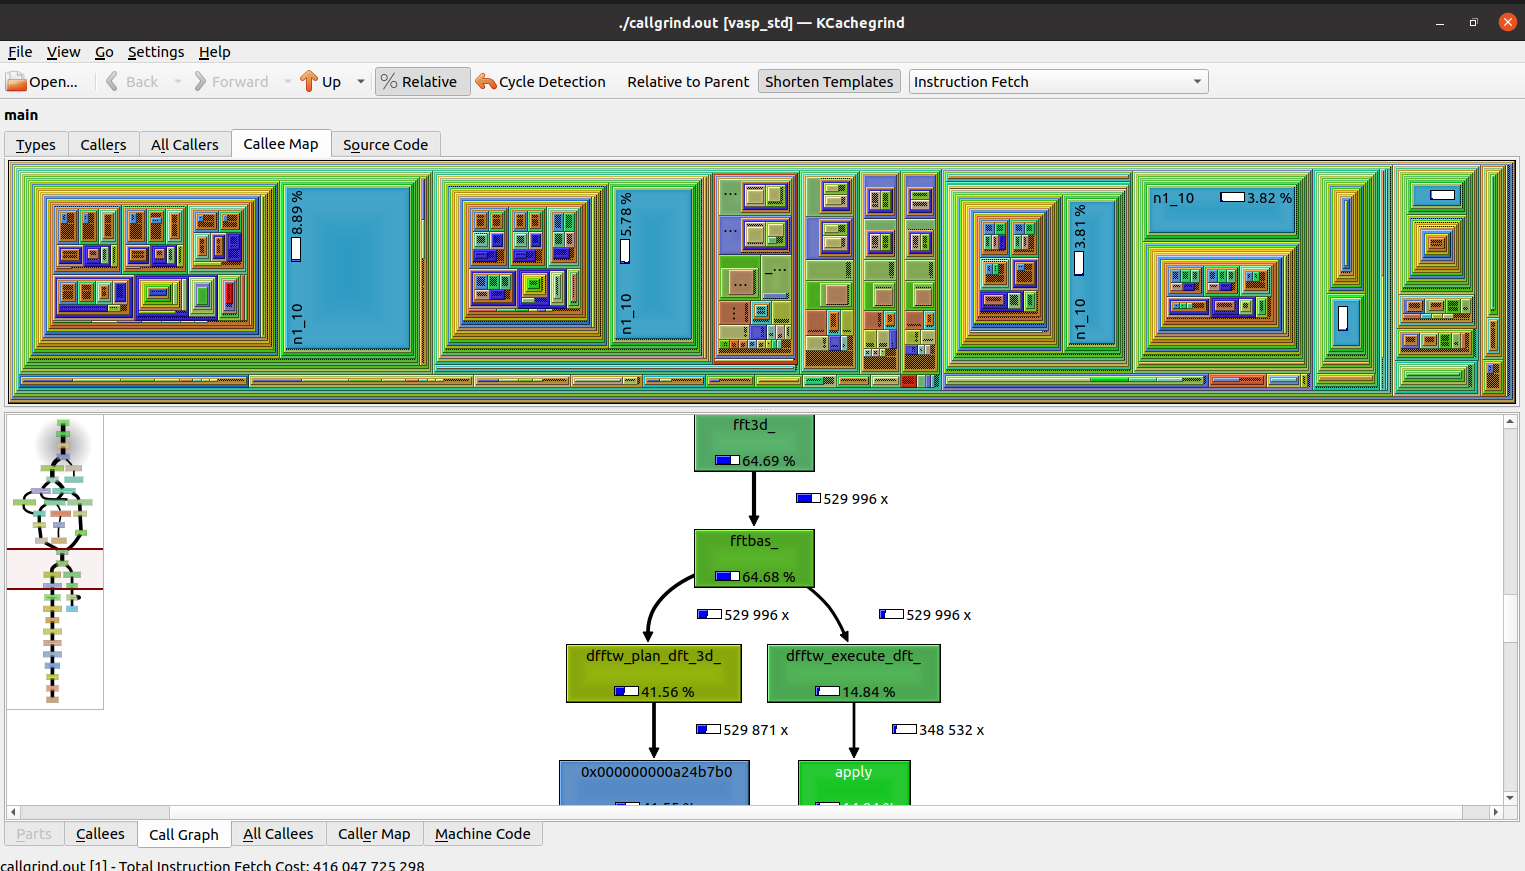
\includegraphics[height=2.5in,width=4.05in,viewport=0 0 1531 877,clip]{Figures/Kcachegrid_analyasis-VASP-05.png}
%%\caption{\tiny \textrm{Compare of VASP calculation with GPU and CPU.}}%(与文献\cite{EPJB33-47_2003}图1对比)
%\label{VASP_Kcachegrind}
%\end{figure} 
%}
%
\frame
{
	\frametitle{双网格技术}
\begin{figure}[h!]
	\vspace{-0.15in}
\centering
%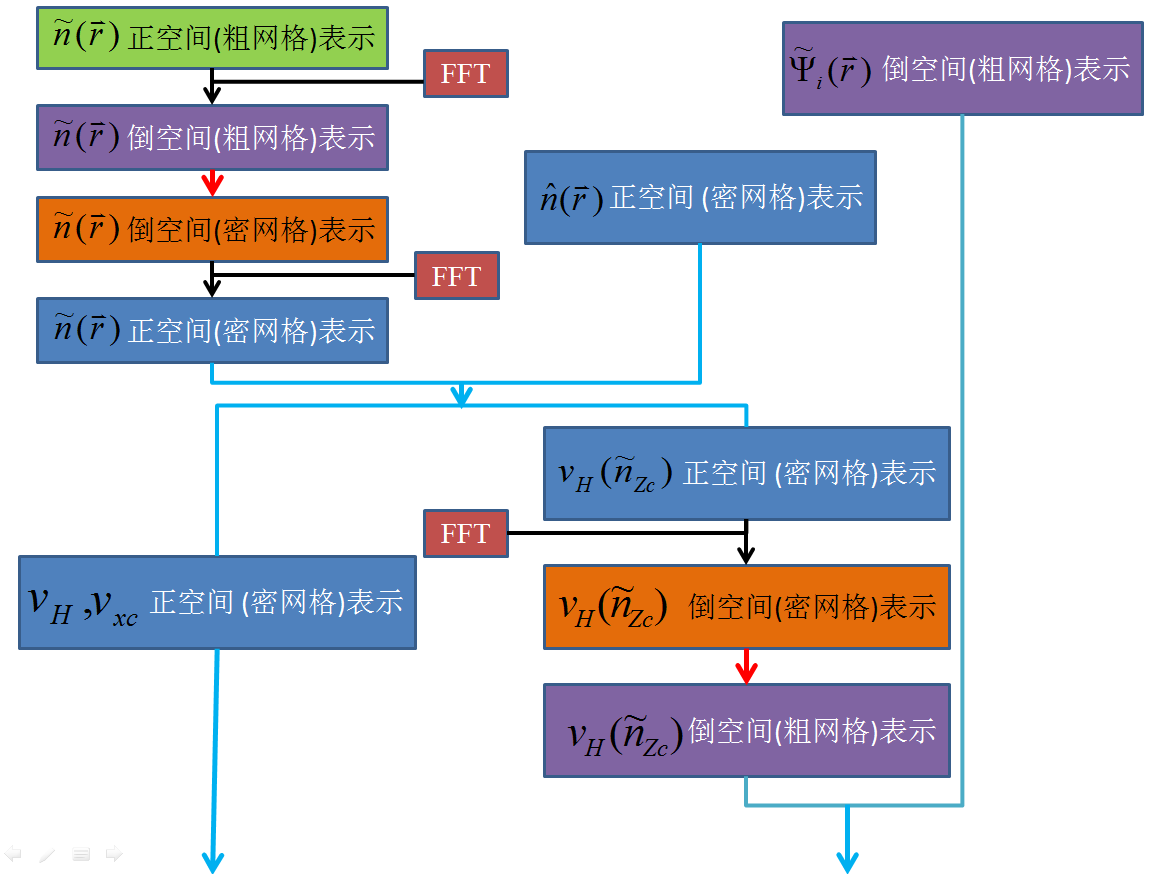
\includegraphics[height=2.7in,width=4.0in,viewport=0 0 1180 875,clip]{Figures/dual_grid.png}
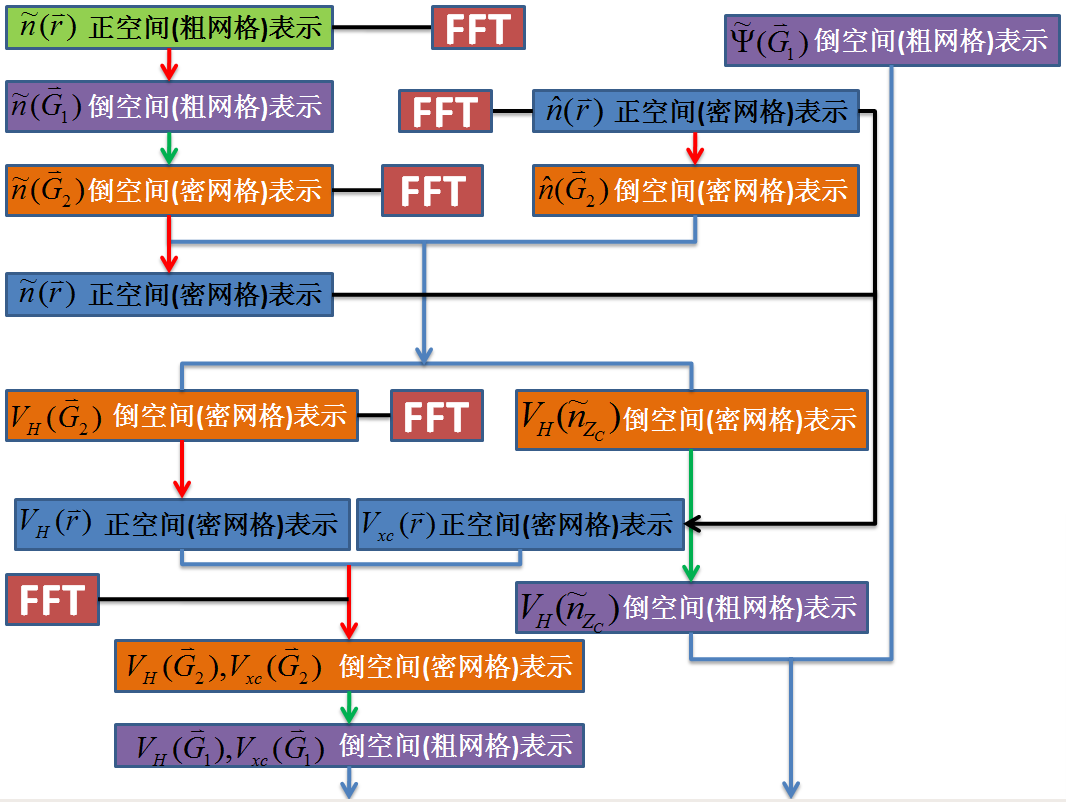
\includegraphics[height=2.75in,width=4.0in,viewport=0 0 800 600,clip]{Figures/dual_grid-2.png}
\caption{\tiny \textrm{The Schematic description of the dual grid technique.}}%(与文献\cite{EPJB33-47_2003}图1对比)
\label{PAW_dualgrid}
\end{figure} 
}

\frame
{
	\frametitle{\textrm{VASP}的并行效率}
	与同类型软件相比,\textrm{VASP}有着优异的并行能力
\begin{figure}[h!]
	\vspace{-0.15in}
\centering
%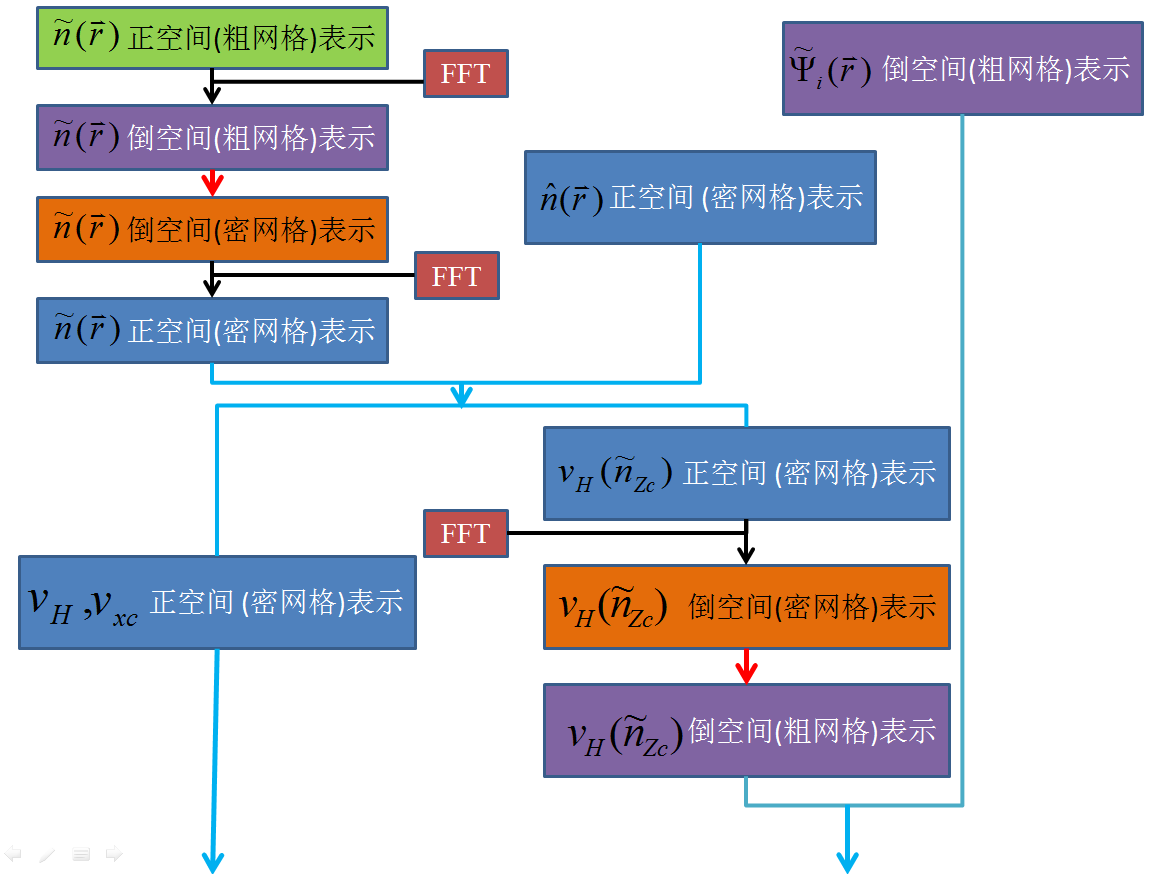
\includegraphics[height=2.7in,width=4.0in,viewport=0 0 1180 875,clip]{Figures/dual_grid.png}
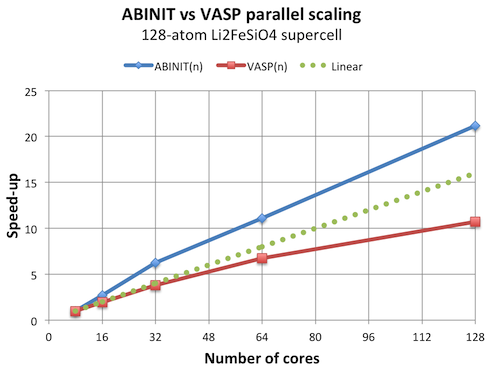
\includegraphics[height=1.55in,width=1.95in,viewport=0 0 240 200,clip]{Figures/VASP-abinit_Li128-1.png}
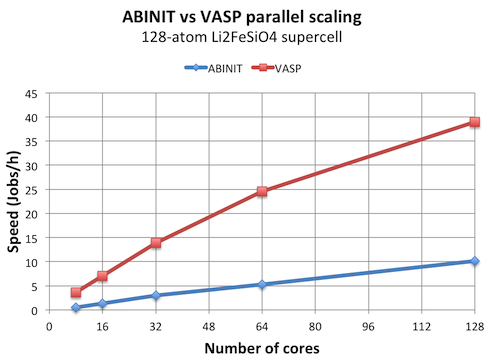
\includegraphics[height=1.55in,width=1.95in,viewport=0 0 240 200,clip]{Figures/VASP-abinit_Li128-2.png}
\caption{\tiny \textrm{The comparison of parallel scaling for ABINIT vs VASP.}}%(与文献\cite{EPJB33-47_2003}图1对比)
\label{ABINIT_vs_VASP}
\end{figure} 
\begin{itemize}
	\item \textrm{VASP}迭代对角化约束了矩阵的维度,减少了对角化过程中的迭代次数,保证了\textrm{MPI}并行的规模和扩展性
	\item \textrm{VASP}实施\textrm{FFT}变换时,保证各节点上处理的网格负载均衡
\end{itemize}
}

\frame
{
	\frametitle{\textrm{VASP}计算的\textrm{FFT}并行实现}
	\begin{itemize}
	     \item 中间层设计:~\textrm{FFT}网格、实空间基组与计算节点的匹配\\
		     \textcolor{red}{通过子程序\textrm{mgrid.F}生成中间层,实现并行负载与计算节点分配的匹配,减少\textrm{FFT}变换和实空间并行的节点间通信}
\begin{figure}[h!]
		\vspace{-0.25in}
	\centering
%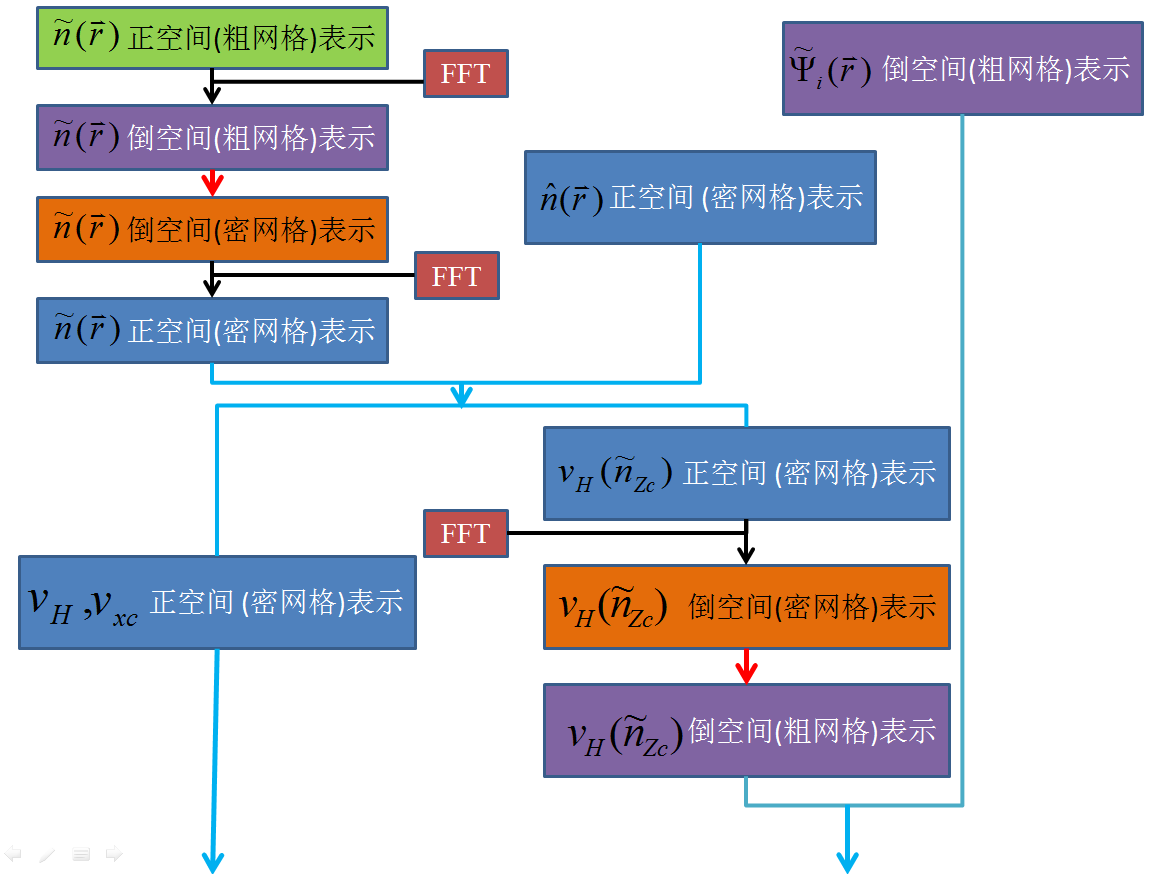
\includegraphics[height=2.7in,width=4.0in,viewport=0 0 1180 875,clip]{Figures/dual_grid.png}
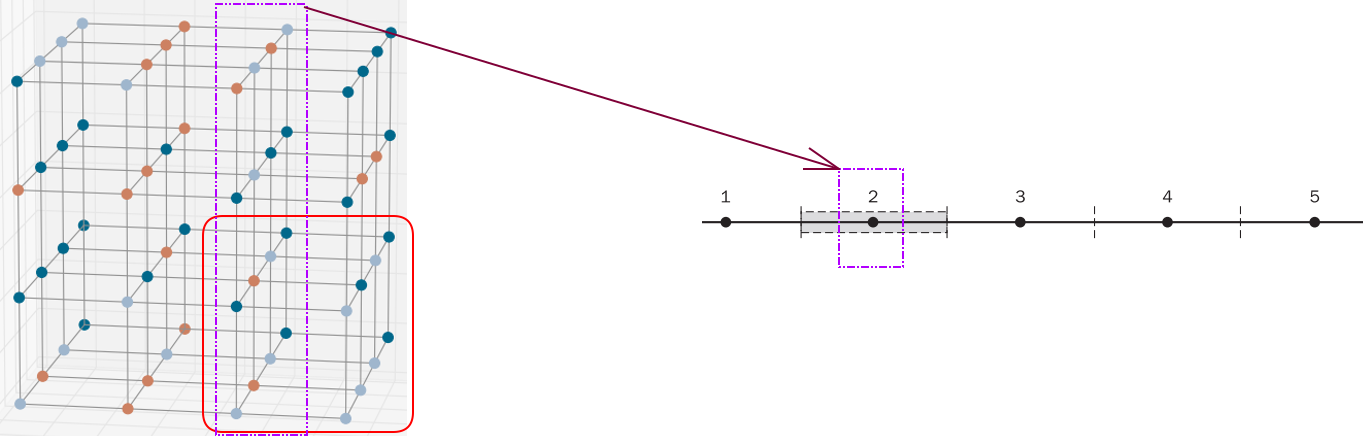
\includegraphics[height=1.0in,width=4.0in,viewport=0 0 1500 450,clip]{Figures/VASP_FFT-MPI_Reciprocal.png}
\vskip 0.5pt
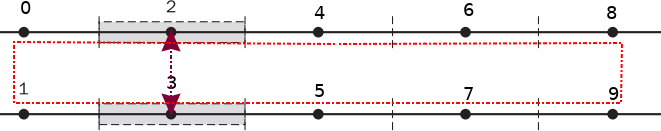
\includegraphics[height=0.7in,width=4.0in,viewport=0 0 730 150,clip]{Figures/VASP_FFT-MPI_Real.png}
\caption{\tiny \textrm{VASP:~ Reciprocal-Real space layout for grids in MPI.}}%(与文献\cite{EPJB33-47_2003}图1对比)
\label{MPI-FFT}
\end{figure} 
	\end{itemize}
}

\frame
{
	\frametitle{\textrm{VASP}的通信开销}
	在高性能的计算队列中,\textrm{VASP}的并行上限可以突破256核,但当并行核数超过百核数量级,并行效率下降非常明显
\begin{figure}[h!]
	\vspace{-0.15in}
\centering
%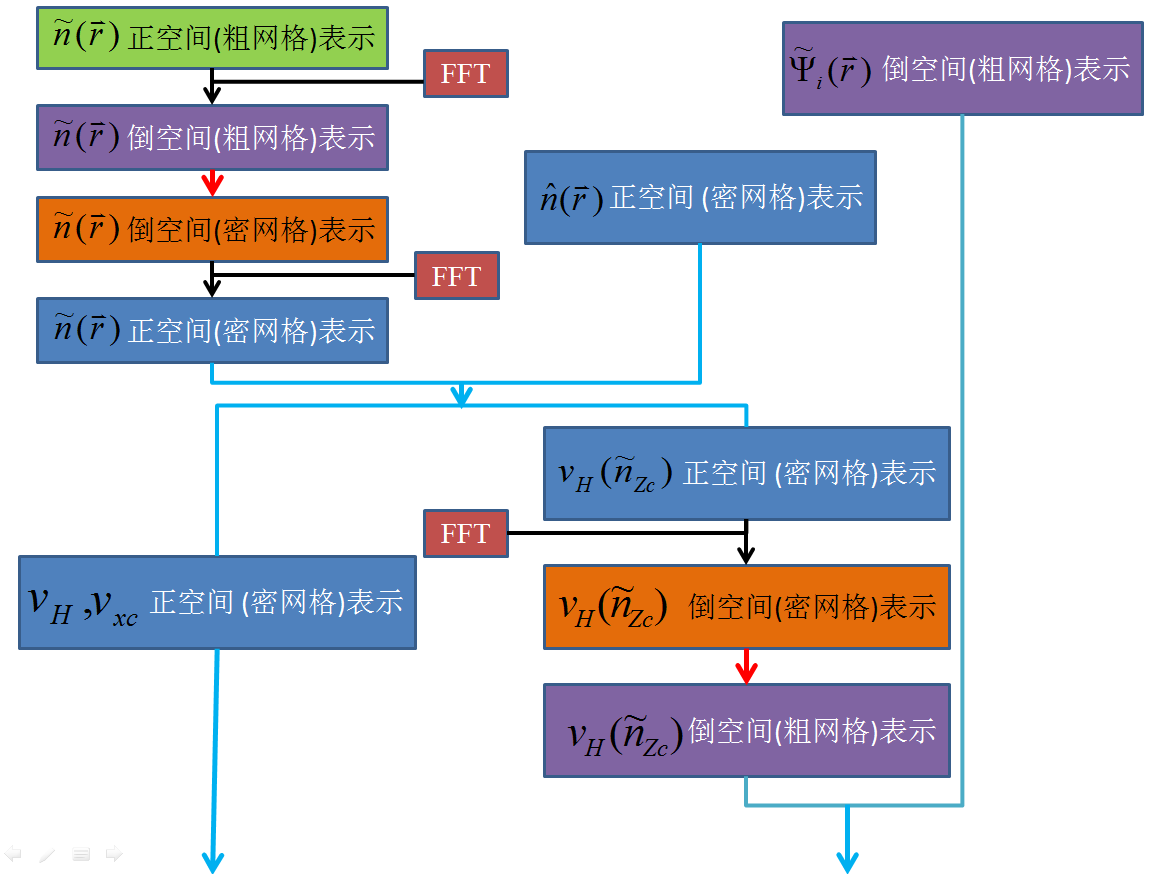
\includegraphics[height=2.7in,width=4.0in,viewport=0 0 1180 875,clip]{Figures/dual_grid.png}
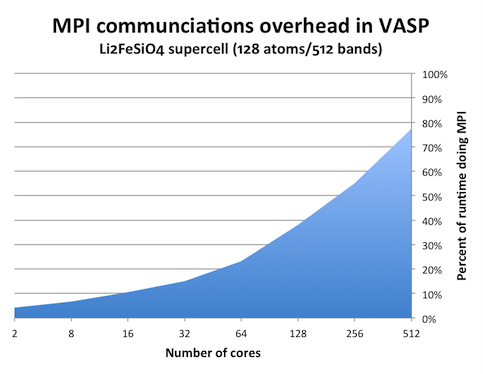
\includegraphics[height=1.55in,width=1.95in,viewport=0 0 240 200,clip]{Figures/VASP-mpi-Li128.png}
\caption{\tiny \textrm{Time spent in MPI calls with increasing the number of ranks in a VASP calculation.}}%(与文献\cite{EPJB33-47_2003}图1对比)
\label{VASP_communication}
\end{figure} 

如能对并行系统与\textrm{VASP}结合作深度改造(如国家超算天津中心方案),\textrm{VASP}的并行扩展可以到$10^4$核级别,但这一改造需要对底层代码和计算框架作较大规模改动
}

\frame
{
	\frametitle{\textrm{VASP}的\textrm{GPU}加速}
\textrm{NVIDIA}多年来致力于\textrm{VASP}的\textrm{GPU}加速,取得了一定的成效
\begin{figure}[h!]
	\vspace{-0.15in}
\centering
%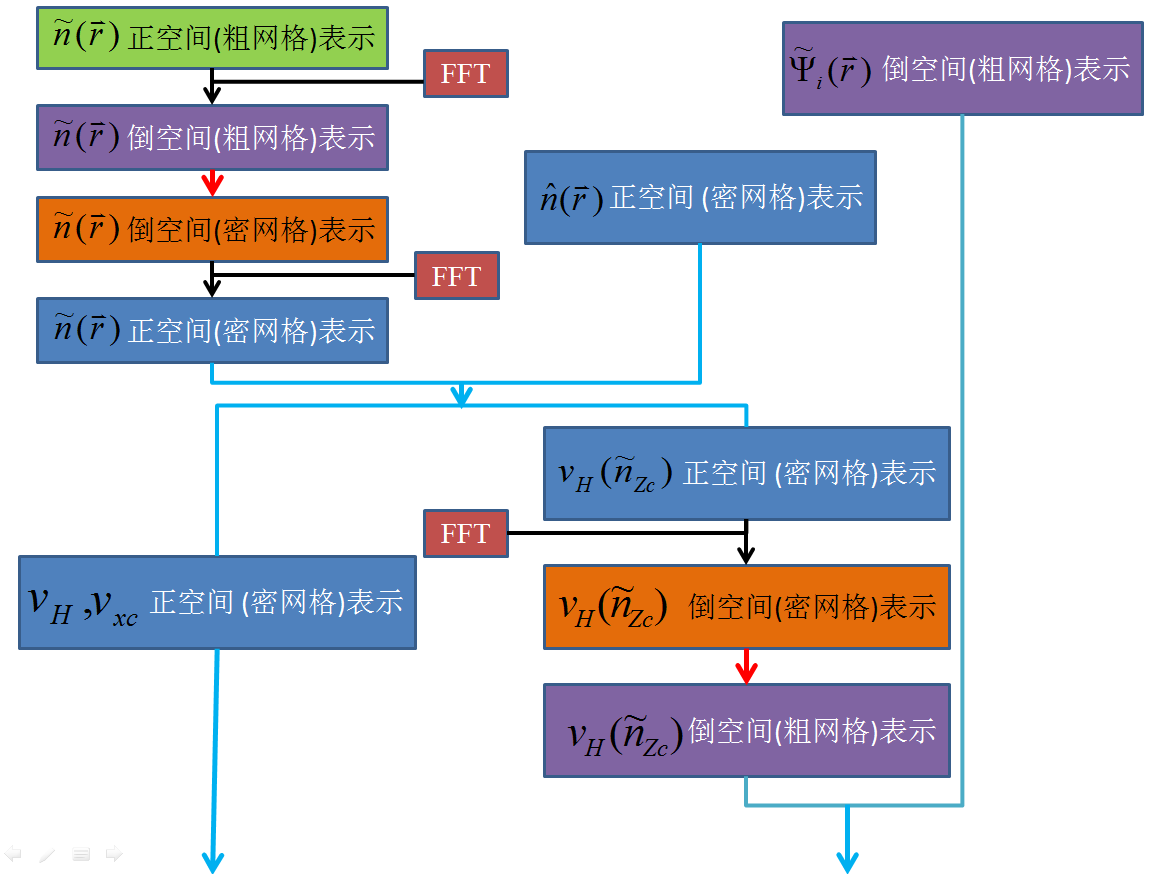
\includegraphics[height=2.7in,width=4.0in,viewport=0 0 1180 875,clip]{Figures/dual_grid.png}
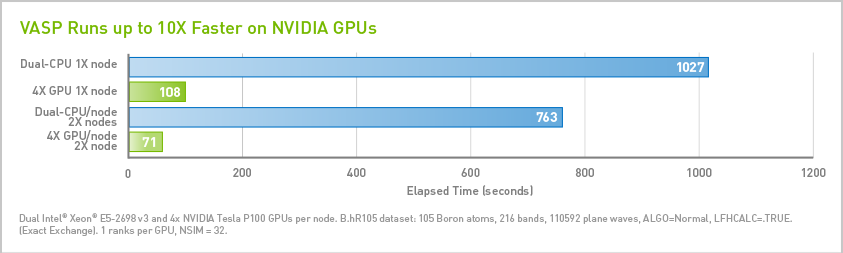
\includegraphics[height=1.2in,width=4.05in,viewport=0 0 850 260,clip]{Figures/VASP-GPU-CPU.png}
\caption{\tiny \textrm{Compare of VASP calculation with GPU and CPU.}}%(与文献\cite{EPJB33-47_2003}图1对比)
\label{VASP_GPU}
\end{figure} 
\begin{itemize}
	\item 通用配置下,\textrm{GPU}对\textrm{VASP}计算有加速效果,一般可提升4$\sim$6倍
	\item 矩阵对角化的并行算法限制了\textrm{GPU}在第一原理计算中的应用
	\item \textrm{GPU}加速的模式主要适合于分子动力学计算
\end{itemize}
}

\frame
{
	\frametitle{\textrm{VASP}的优化算法}
	与其余第一原理计算软件相比,\textrm{VASP}的最大优势
	\begin{itemize}
		\item 提供了多种电子结构和原子受力的优化算法(\textrm{SD}、\textrm{CG}、\textrm{RMM-DIIS}等)\\
			用户可以通过控制文件\textcolor{blue}{\textrm{INCAR}}的参数调控来选择
		\item 提供了基于\textrm{PAW}方法适用性广泛的原子数据集文件\textrm{POTCAR}
	\begin{itemize}
		\item \textrm{POTCAR}是\textrm{VASP}实现材料精确计算的重要保证\\
			同样都应用\textrm{PAW}方法,\textcolor{blue}{公认\textrm{VASP}较\textrm{QE}、\textrm{ABINIT}等软件的计算精度要高}
		\item \textrm{POTCAR}数据生成依赖较多的可调参数\\
			包括能量参数$\varepsilon_l$、多种截断半径$r_c$、$r_{\mathrm{vloc}}$、$r_{\mathrm{shape}}$、$r_{\mathrm{core}}$
		\item \textcolor{red}{\textrm{POTCAR}数据生成代码是\textrm{VASP}中唯一没有公开的}
%		\item 用\textrm{VASP}模拟极端条件下材料物性的能力,受到\textrm{POTCAR}数据的制约
	\end{itemize}
	\end{itemize}
}


\frame
{
	\frametitle{\textrm{PAW}原子数据集:~\textrm{wave~function}}
	平滑赝原子分波函数
	\begin{displaymath}
		\tilde\phi_{i=Lk}(\vec r)=Y_L(\widehat{\vec r-\vec R})\tilde\phi_{lk}(|\vec r-\vec R|)
	\end{displaymath}
	根据\textrm{RRKJ}赝势构造的思想,赝分波函数由球\textrm{Bessel}函数线性组合%\upcite{JPCM6-8245_1994}
	\begin{displaymath}
		\tilde\phi_{lk}(r)=\left\{
		\begin{aligned}
			&\sum_{i=1}^2\alpha_ij_l(q_ir)\quad &r<r_c^l\\
			&\phi_{lk}(r)\quad&r>r_c^l
		\end{aligned}
		\right.
	\end{displaymath}
	调节系数$\alpha_i$和$q_i$赝分波函数$\phi_{lk}(r)$在截断半径$r_c^l$处两阶连续可微
%	投影子波函数$\tilde p_i$由\textrm{Gram-Schmidt}正交条件$\langle\tilde p_i|\tilde\phi_j\rangle=\delta_{ij}$确定
}

\frame
{
	\frametitle{\textrm{PAW}原子数据集:~\textrm{wave~function}}
\begin{figure}[h!]
\centering
\vskip -0.5in
\includegraphics[width=1.5in,height=2.7in,viewport=0 0 350 550, angle=-90, clip]{Figures/WAE-data.eps}
\vskip -0.2in
\includegraphics[height=2.7in,width=1.5in,viewport=0 0 350 550, angle=-90, clip]{Figures/WPS-data.eps}
\caption{\tiny \textrm{The partial wave function.}}%(与文献\cite{EPJB33-47_2003}图1对比)
\label{Wave_Function}
\end{figure}
}

\frame
{
	\frametitle{\textrm{PAW}原子数据集:~\textrm{core~density}}
	\textcolor{blue}{构造赝芯电荷密度$\tilde n_c$}:~在截断半径$r_{\mathrm{core}}$内的定义为
	$$\sum_{i=1,2}B_i\dfrac{\sin(q_ir)}r\quad r<r_{\mathrm{core}}$$
	调节系数$q_i$和$B_i$使得赝芯电荷密度$\tilde n_c(r)$在截断半径$r_{\mathrm{core}}$处的两阶导数连续
\begin{figure}[h!]
\vskip -0.5in
\centering
\hspace*{-0.1in}
\includegraphics[width=1.5in,height=2.35in,viewport=0 0 350 550, angle=-90, clip]{Figures/CORE-data.eps}
\hspace*{-0.7in}
\includegraphics[height=2.35in,width=1.5in,viewport=0 0 350 550, angle=-90, clip]{Figures/PCORE-data.eps}
\caption{\tiny \textrm{The core density.}}%(与文献\cite{EPJB33-47_2003}图1对比)
\label{core_density_Function}
\end{figure}
}

\frame
{
	\frametitle{\textrm{PAW}原子数据集:~$\mathrm{v}_{e\!f\!f}(r)$与$\tilde{\mathrm{v}}_{e\!f\!f}(r)$}
	\textcolor{blue}{原子局域有效势$\mathrm{v}_{e\!f\!f}^a$}
\begin{figure}[h!]
%\vskip -0.5in
\vskip -0.17in
\centering
%\includegraphics[width=1.6in,height=2.7in,viewport=0 0 300 460, angle=-90, clip]{Figures/POTAE-data.eps}
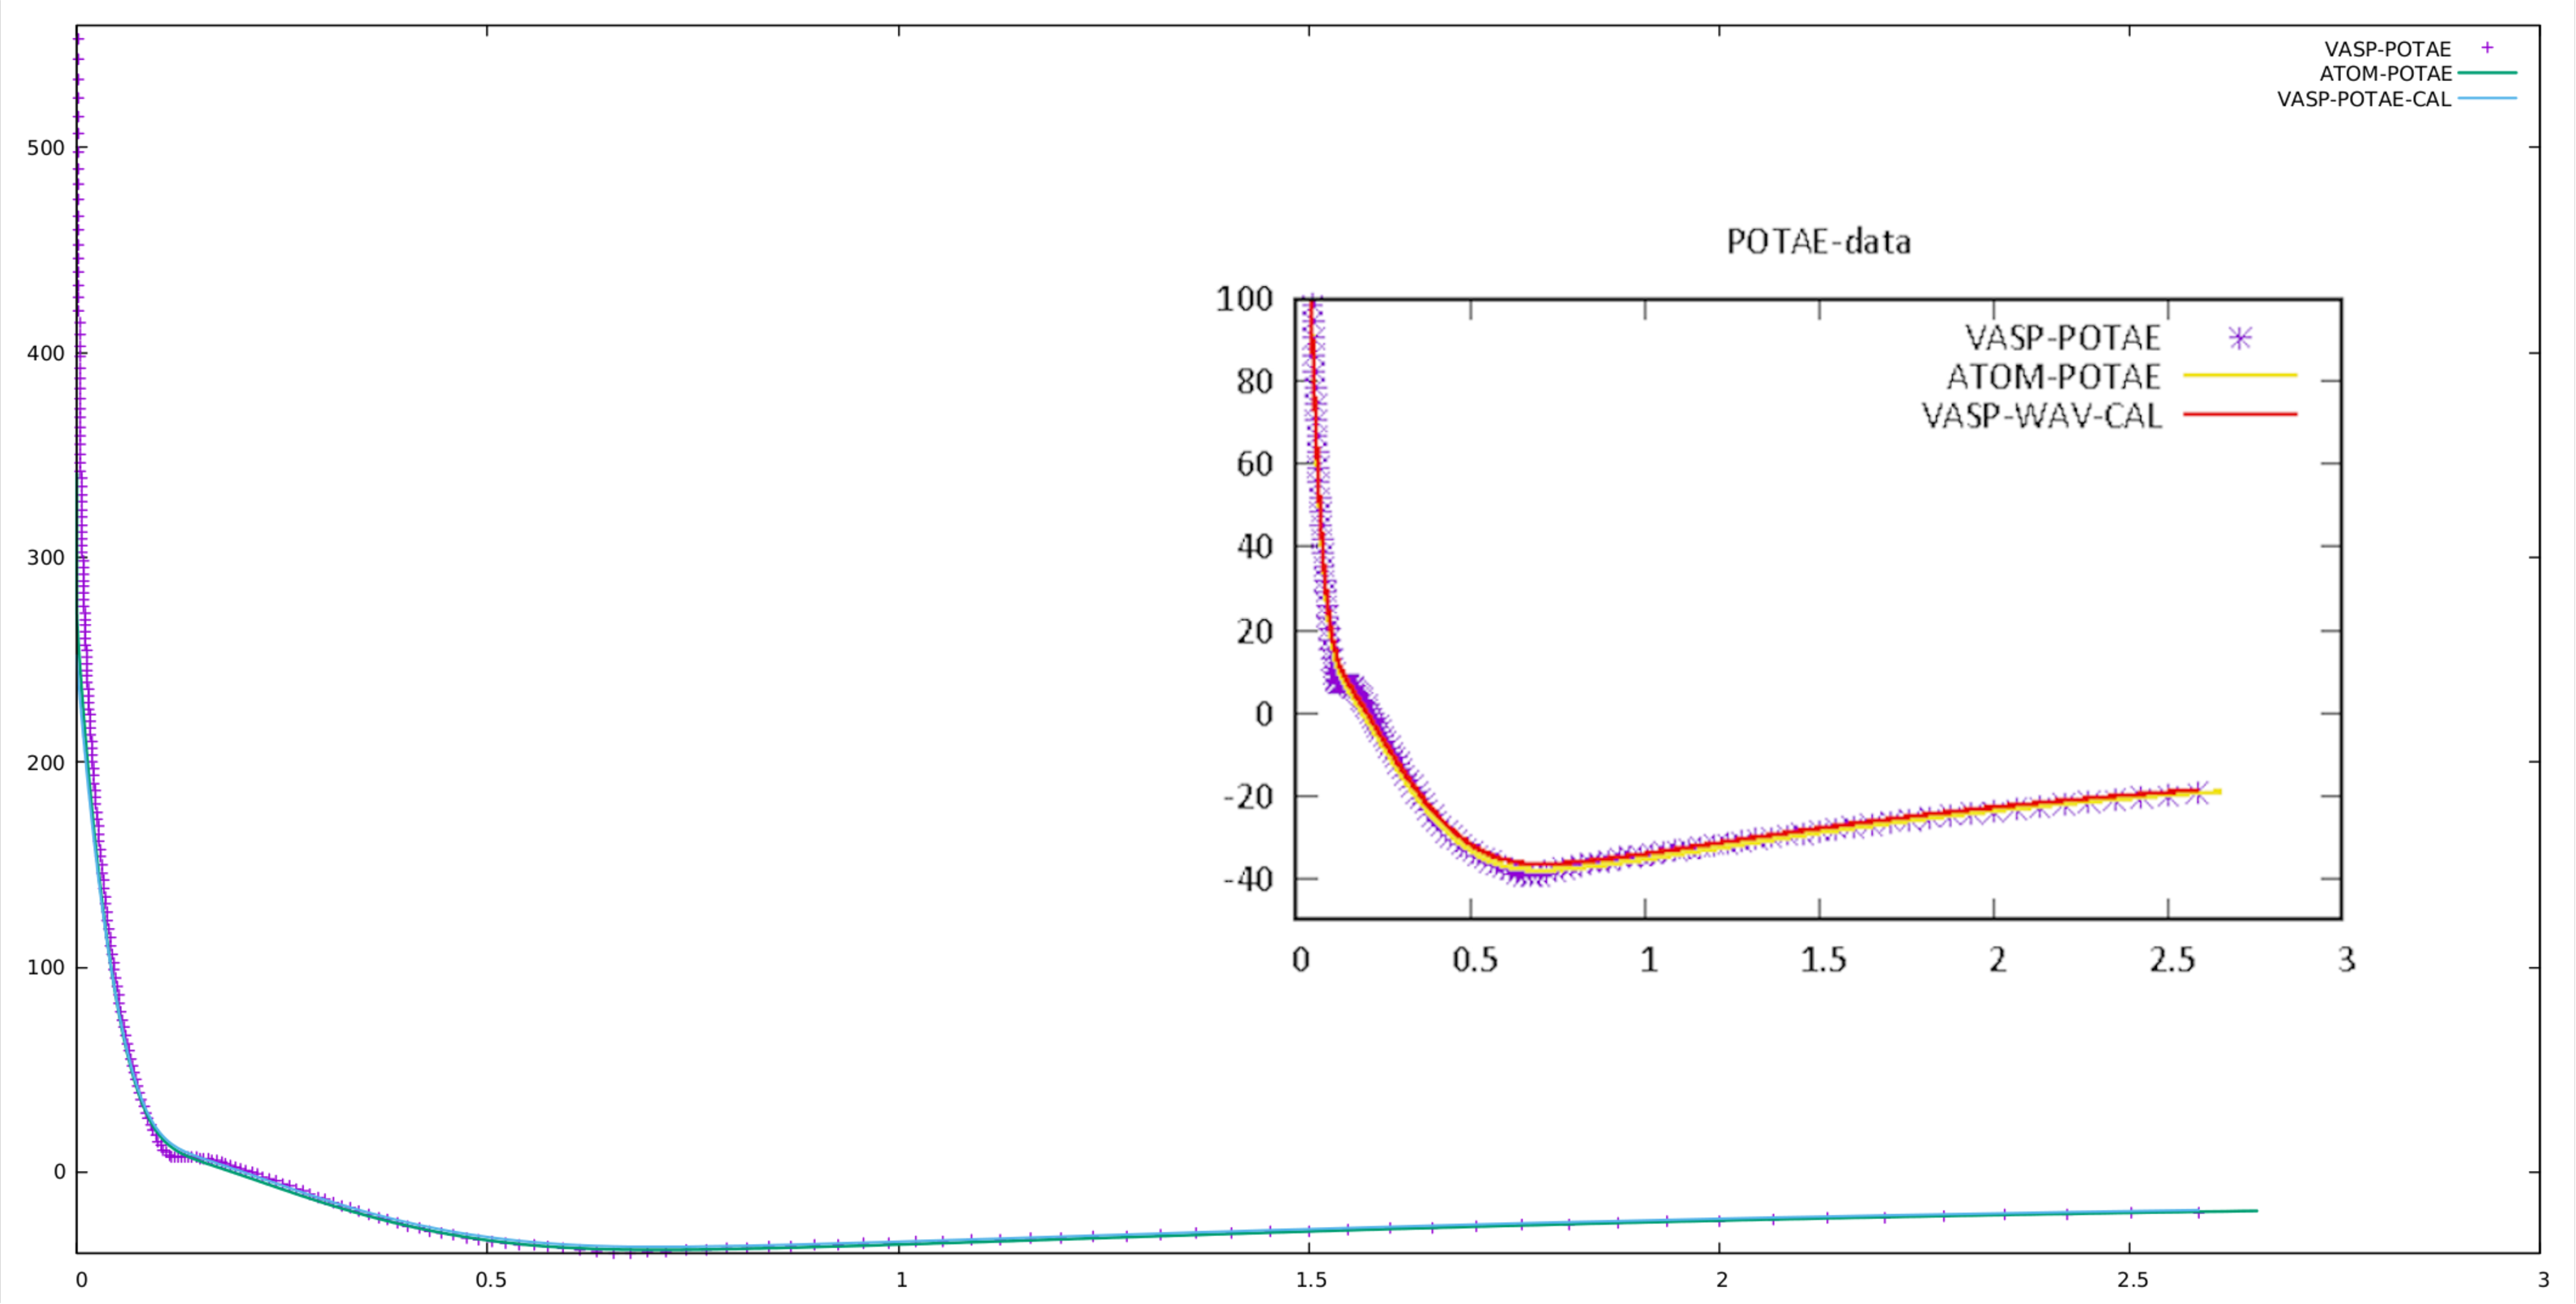
\includegraphics[width=2.5in,height=1.2in,viewport=0 0 1600 800, clip]{Figures/POTAE-full-dat.pdf}
\caption{\tiny \textrm{The local atomic effective-Potential.}}%(与文献\cite{EPJB33-47_2003}图1对比)
\label{local_atomic_PP}
\end{figure}
	\textcolor{blue}{构造原子局域赝势$\tilde v_{e\!f\!f}^a$}%(\textcolor{red}{为防止\textrm{ghost band}})
	:%\\
	(在截断半径$r_{\mathrm{loc}}$内的定义)
	$$\tilde v_{e\!f\!f}^a=A\dfrac{\sin(q_{loc}r)}r\quad r<r_{\mathrm{loc}}$$
	其中$q_{loc}$和$A$要求局域赝势在截断半径$r_{\mathrm{loc}}$处连续到一阶导数
}

\frame
{
	\frametitle{\textrm{PAW}原子数据集:~$\mathrm{v}_H[\tilde n_{Zc}]$}
	局域离子赝势$v_H[\tilde n_{Zc}]$可由原子局域赝势去屏蔽得到
	$$v_H[\tilde n_{Zc}]=\tilde v_{e\!f\!f}^a-v_H[\tilde n_a^1+\hat n_a]-v_{\mathrm{XC}}[\tilde n_a^1+\hat n_a+\tilde n_c]$$
\begin{figure}[h!]
\vskip -0.5in
\centering
\hspace*{-0.1in}
\includegraphics[width=1.5in,height=2.35in,viewport=0 0 350 550, angle=-90, clip]{Figures/POTPS-data.eps}
\hspace*{-0.7in}
\includegraphics[height=2.35in,width=1.5in,viewport=0 0 350 550, angle=-90, clip]{Figures/POTPSC-data.eps}
\caption{\tiny \textrm{The pseudo-potential and local ionic pseudo-potential.}}%(与文献\cite{EPJB33-47_2003}图1对比)
\label{pseudo_potential}
\end{figure}
}

\frame
{
	\frametitle{\textrm{PAW}原子数据集:~$\tilde{n}_{\mathrm G}$}
	局域离子赝势$\tilde{n_{\mathrm G}}$可由原子局域赝密度的\textrm{FFT}得到
\begin{figure}[h!]
\vskip -0.2in
\centering
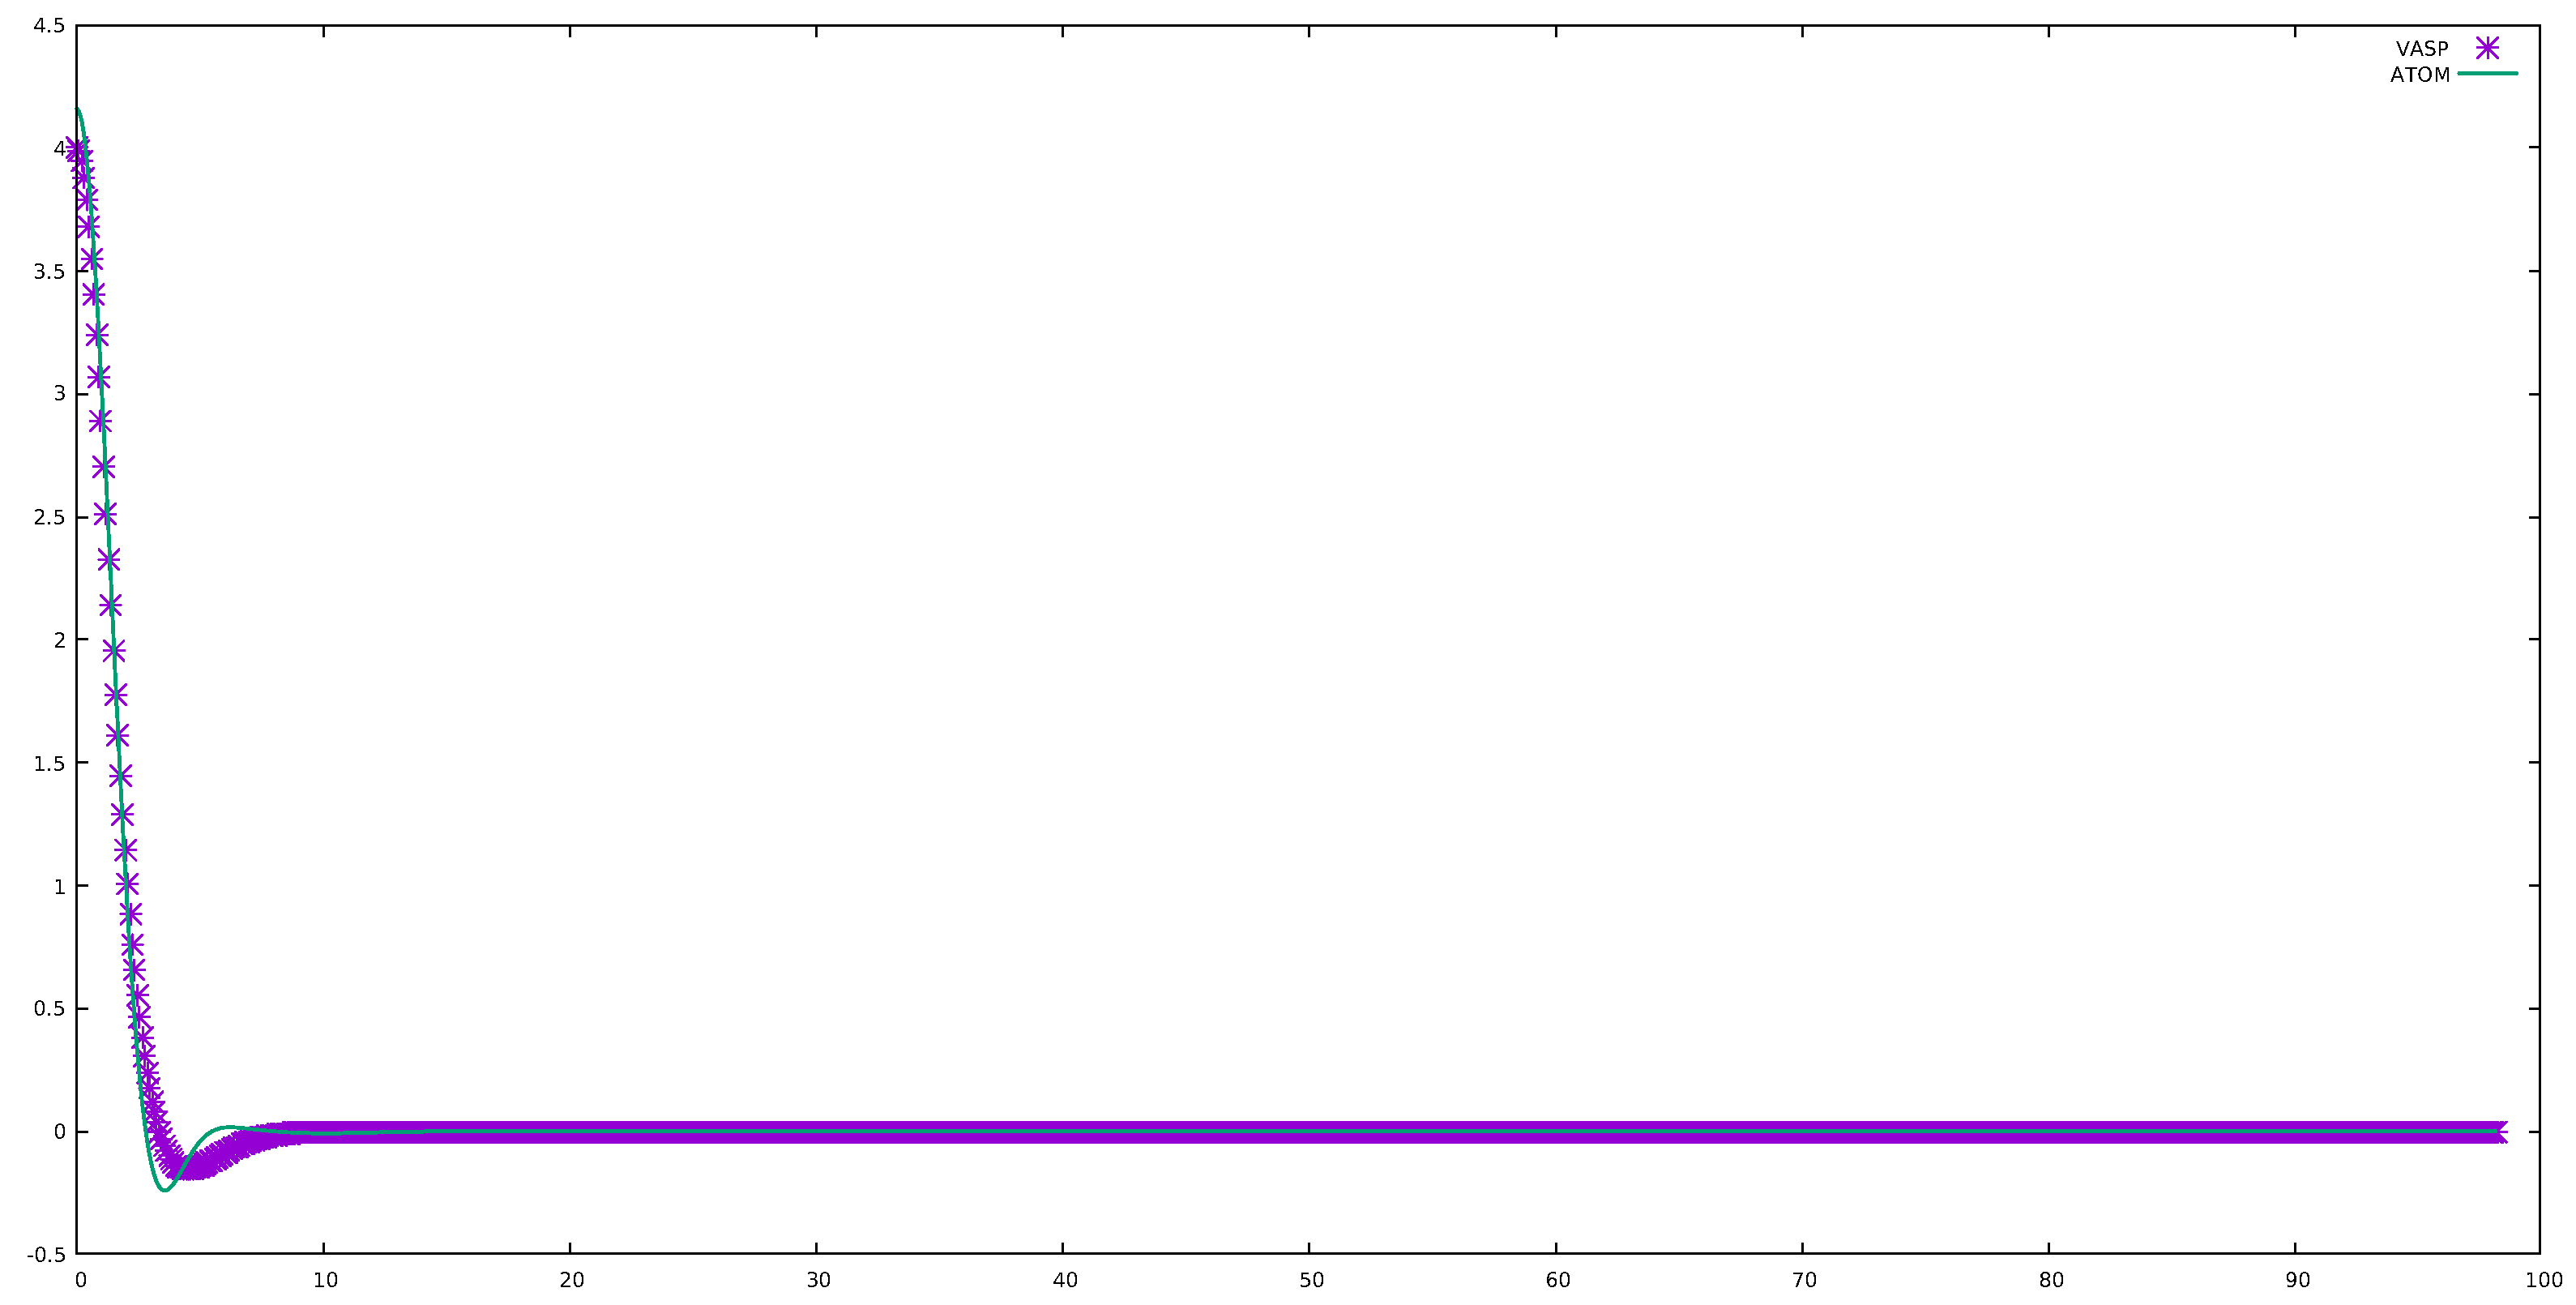
\includegraphics[width=4.0in,height=2.35in,viewport=0 0 1530 850, clip]{Figures/PSRHO_G-dat.pdf}
\caption{\tiny \textrm{The pseudo-density in reciprocal space.}}%(与文献\cite{EPJB33-47_2003}图1对比)
\label{pseudo_density_in_reciprocal-space}
\end{figure}
}

\frame
{
	\frametitle{\textrm{PAW}原子数据集:~$\mathrm{v}_{\mathrm G}[\tilde n_{Zc}]$}
	局域离子赝势在倒空间的表示$v_{\mathrm G}[\tilde n_{Zc}]$可由原子去屏蔽局域赝势的\textrm{FFT}得到
\begin{figure}[h!]
\vskip -0.2in
\centering
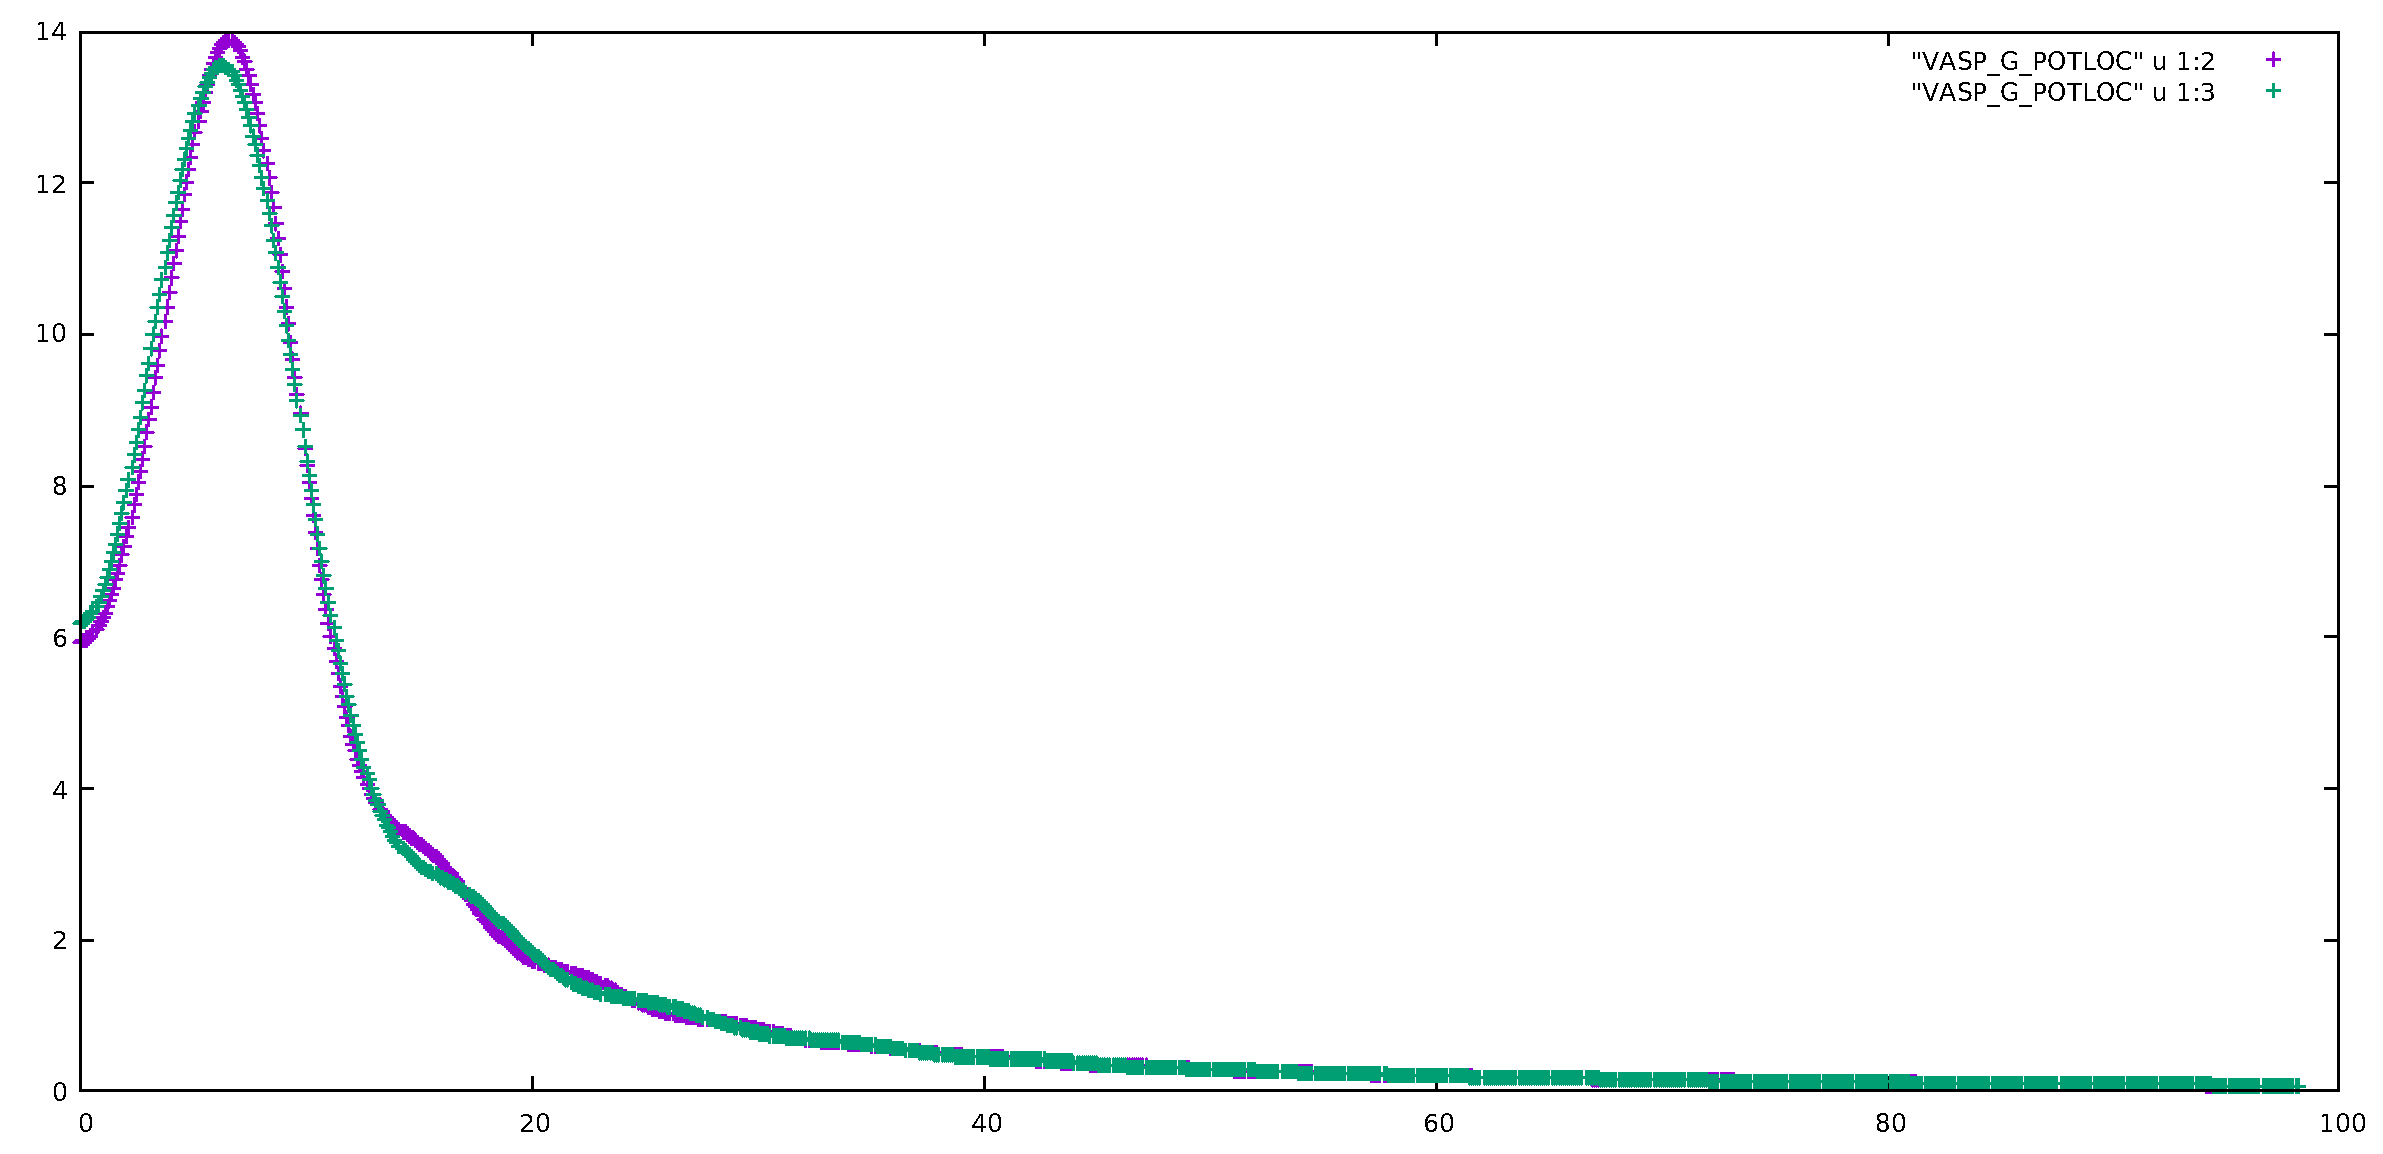
\includegraphics[width=4.0in,height=2.35in,viewport=0 0 1150 650, clip]{Figures/POT_G-dat.pdf}
\caption{\tiny \textrm{The local ionic pseudo-potential in reciprocal space.}}%(与文献\cite{EPJB33-47_2003}图1对比)
\label{pseudo_potential_in_reciprocal-space}
\end{figure}
}

\frame
{
	\frametitle{小结}
	作为第一性原理计算的商用软件,\textrm{VASP}已成为计算材料学领域应用最广泛的软件之一。全球绝大多数超算中心都安装了\textrm{VASP},据统计,\textrm{VASP}软件的作业机时占用全球总机时的12$\sim$20\%,但由于其%类似于linpack软件,
属于重型浮点计算密集型应用,实际耗电量占比则高达30$\sim$50\%
\vskip 3pt
	{\fontsize{9.0pt}{7.2pt}\selectfont{
	\begin{itemize}
\setlength{\itemsep}{5pt}
		\item \textcolor{blue}{物理上},\textrm{VASP}基于\textrm{DFT}近似,求解\textrm{Kohn-Sham}方程,并将粒子基态密度问题转化为矩阵的本征函数和本征值问题
		\item \textcolor{blue}{数学上},方程求解过程的核心是矩阵对角化与\textrm{PDE}的自洽迭代,即便对于简单体系,也需要完成数十次的迭代,而规模大的计算模拟体系则可能需要成千上万次迭代计算
		\item \textcolor{blue}{计算过程上},\textrm{VASP}计算的时长开销主要是本征值求解的矩阵对角化;此外由于算法限制,\textrm{Kohn-Sham}方程作为线性方程组作并行处理时,节点间存在密集的通信。在上千节点,上万计算核的大规模并行系统上,数据通信将严重影响程序的性能,这是当前\textrm{VASP}软件的主要瓶颈
	\end{itemize}}}
%			\textcolor{magenta}{有必要探索新的并行和优化策略来提升\textrm{VASP}的计算性能}
}
